\documentclass[11pt]{article}\usepackage[]{graphicx}\usepackage[]{color}
%% maxwidth is the original width if it is less than linewidth
%% otherwise use linewidth (to make sure the graphics do not exceed the margin)
\makeatletter
\def\maxwidth{ %
  \ifdim\Gin@nat@width>\linewidth
    \linewidth
  \else
    \Gin@nat@width
  \fi
}
\makeatother

\definecolor{fgcolor}{rgb}{0, 0, 0}
\newcommand{\hlnum}[1]{\textcolor[rgb]{0,0,0}{#1}}%
\newcommand{\hlstr}[1]{\textcolor[rgb]{0,0,0}{#1}}%
\newcommand{\hlcom}[1]{\textcolor[rgb]{0.4,0.4,0.4}{\textit{#1}}}%
\newcommand{\hlopt}[1]{\textcolor[rgb]{0,0,0}{\textbf{#1}}}%
\newcommand{\hlstd}[1]{\textcolor[rgb]{0,0,0}{#1}}%
\newcommand{\hlkwa}[1]{\textcolor[rgb]{0,0,0}{\textbf{#1}}}%
\newcommand{\hlkwb}[1]{\textcolor[rgb]{0,0,0}{\textbf{#1}}}%
\newcommand{\hlkwc}[1]{\textcolor[rgb]{0,0,0}{\textbf{#1}}}%
\newcommand{\hlkwd}[1]{\textcolor[rgb]{0,0,0}{\textbf{#1}}}%
\let\hlipl\hlkwb

\usepackage{framed}
\makeatletter
\newenvironment{kframe}{%
 \def\at@end@of@kframe{}%
 \ifinner\ifhmode%
  \def\at@end@of@kframe{\end{minipage}}%
  \begin{minipage}{\columnwidth}%
 \fi\fi%
 \def\FrameCommand##1{\hskip\@totalleftmargin \hskip-\fboxsep
 \colorbox{shadecolor}{##1}\hskip-\fboxsep
     % There is no \\@totalrightmargin, so:
     \hskip-\linewidth \hskip-\@totalleftmargin \hskip\columnwidth}%
 \MakeFramed {\advance\hsize-\width
   \@totalleftmargin\z@ \linewidth\hsize
   \@setminipage}}%
 {\par\unskip\endMakeFramed%
 \at@end@of@kframe}
\makeatother

\definecolor{shadecolor}{rgb}{.97, .97, .97}
\definecolor{messagecolor}{rgb}{0, 0, 0}
\definecolor{warningcolor}{rgb}{1, 0, 1}
\definecolor{errorcolor}{rgb}{1, 0, 0}
\newenvironment{knitrout}{}{} % an empty environment to be redefined in TeX

\usepackage{alltt}
\usepackage{fullpage,graphicx,float,amsmath,enumitem,hyperref}
\setlist{parsep=5.5pt}
\setlength{\parindent}{0pt}
\setlength{\parskip}{\baselineskip}

\usepackage{fancyhdr}
\pagestyle{fancy}
\lhead{Missing Data and LOD}
\rhead{Paul Harmon, Nnamdi Ezike, and Andrea Mack}
\setlength{\headheight}{18pt}
\setlength{\headsep}{2pt}

\title{Pea Lodging Final Report}
\author{Client: Jamin Smitchger\\
Consultants: Paul Harmon, Nnamdi Ezike, and Andrea Mack}
\date{December 16, 2016}
\IfFileExists{upquote.sty}{\usepackage{upquote}}{}
\begin{document}
\maketitle





\section{Introduction}
Jamin is a Ph.D. student in the Department of Plant Sciences and Plant Pathology at MSU. The primary focus is his research is to associate variation in genetic expression with variation in the expression of several phenotypic traits. Genotypic and pheynotypic data were collected on 257 varieties of pea, from two locations (Bozeman and Moccasin), over 4 years. Phenotypic data includes percent lodging, tendril length, tendril node length, nodes at 1st flow, maximum number of nodes, germination, number of branches, plant height, plant length, average total yield, main stem diameter, tiller diameter, ``comp" tiller diameter, and maturation time, totaling 14 traits. Data from 609 genetic markers were collected. The end result of Jamin's research will include a quantitative trait loci (QTL) analysis. Prior to the QTL analysis, understanding of the data and methods are necessary. The report includes:

\begin{itemize}

\item Evaluation of correlations in pheynotypic data

\item Analysis of combining data from the different sites and years

\item Exploration of the rate of missing data

\item Explanation of significance thresholds for QTL 

\item Suggestions for future work
\end{itemize}
\pagebreak

\section{Correlation Plots}
Correlation describes the strength and direction of a linear association. Specifically, this analysis examines Pearson Correlations because the variables are measured on a quantitative scale.  Correlation is measured on a scale between -1 (a perfect negative linear association) and 1 (a perfect positive linear association). Correlation does not imply causal relationships. In examining, for instance, the relationship between lodging and stem width, the Pearson Correlation would only give information about the linear association between the two variables.  A strong association between the two variables cannot be interpreted as stem width causes lodging; rather, we would simply say that the two variables are associated with each other. Other confounding variables, such as climate, may be driving both. Since the phenotypes in each year at each site are considered separate response values, we consider fitting correlation plots for each site/year combination as well as for the entire dataset. 

\subsection{Sites and Years Combined}
The correlation between pairwise explanatory variables of the phenotypic data were assessed using the a pairwise correlation matrix. We assessed the pairwise correlations across sites for pairs of explanatory variables which were measured within these sites at least in two different years.

In Moccasin, only four variables were observed to have been measured both in 2015 and 2016. Of these variables, the length and main stem diameter of the plants are moderately correlated (r=-0.55). Also, the main stem diameter and root diameter of the plants are moderately correlated (r=0.45).
\pagebreak
\subsection{Bozeman in All Years}
The pairwise correlation matrix below shows that germination which was measured in Bozeman for all 3 years has weak correlation against all the variables measured. Also results from Bozeman shows that tendril length node of the plant was moderately to strongly correlated with the average length and tendril length of the plant with correlation coefficients of 0.61 and 0.48 respectively. The branch number and tiller diameter of the plant were also moderately correlated (r = 0.47). The maturity time of the plant was strongly and moderately correlated with the maximum nodes (r=0.65) and nodes of 1st flow (r=0.48). In addition, a correlation coefficient of 0.81 was observed for nodes 1st flow and maximum nodes of the plants.

\begin{knitrout}\footnotesize
\definecolor{shadecolor}{rgb}{1, 1, 1}\color{fgcolor}

{\centering 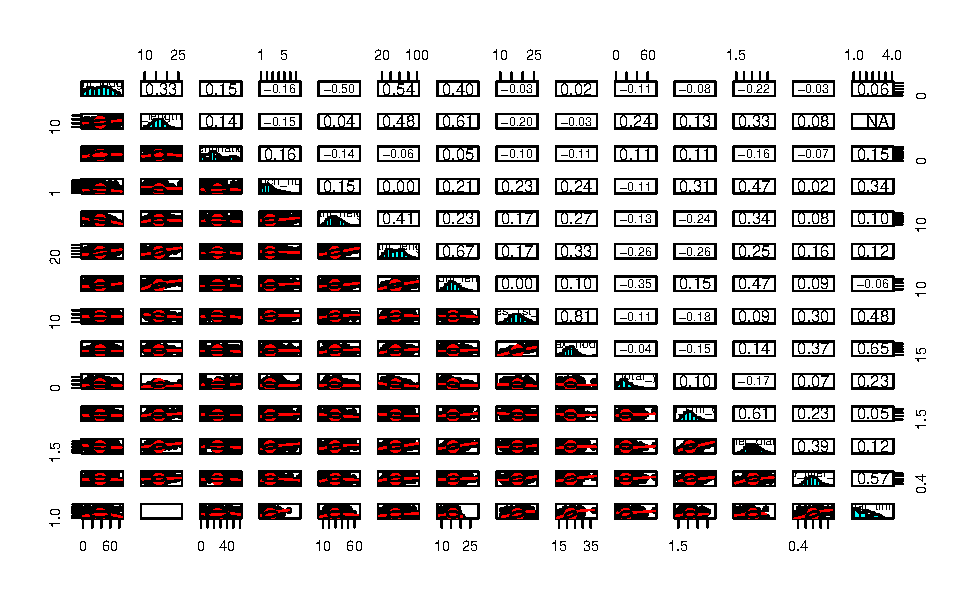
\includegraphics[width=\maxwidth]{figure/merged-1} 

}



\end{knitrout}




\subsection{Bozeman by Year}
We assessed the pairwise correlation of the different sites each year. In 2014, twelve pairs of explanatory variables had correlation coefficients between 0.42 and 0.91. The pairwise correlations are shown in the matrix below. Germination and total yield was strongly correlated (r=0.66) while the length and internode length of the plants recorded a very high correlation coefficient (r=0.91). In 2015 and 2016, of the pairwise combinations assessed, 28 combinations yielded correlation coefficients between 0.40 and 0.85. The results are presented in the pairwise correlation matrices below.

\begin{knitrout}\footnotesize
\definecolor{shadecolor}{rgb}{1, 1, 1}\color{fgcolor}

{\centering 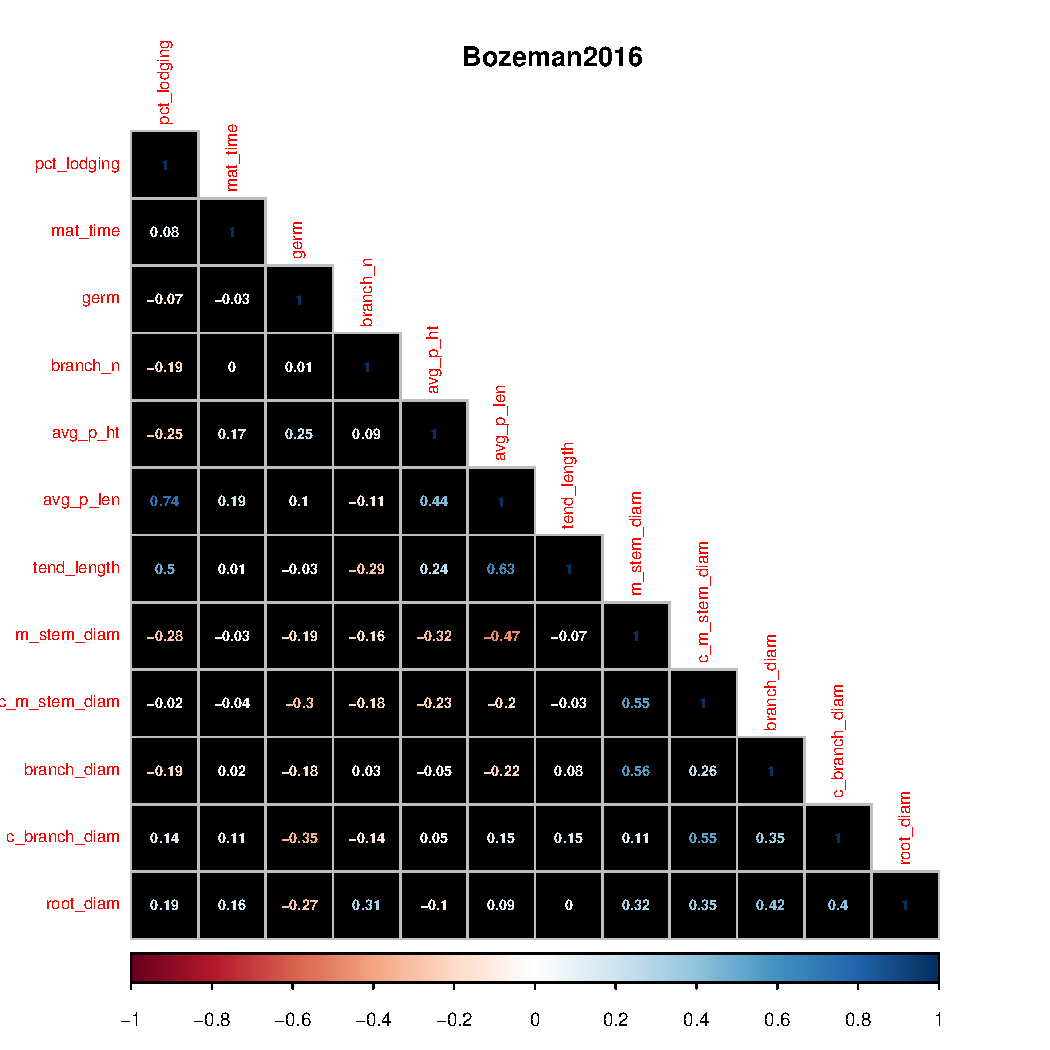
\includegraphics[width=\maxwidth]{figure/bz-1} 

}



\end{knitrout}

\begin{knitrout}\footnotesize
\definecolor{shadecolor}{rgb}{1, 1, 1}\color{fgcolor}

{\centering 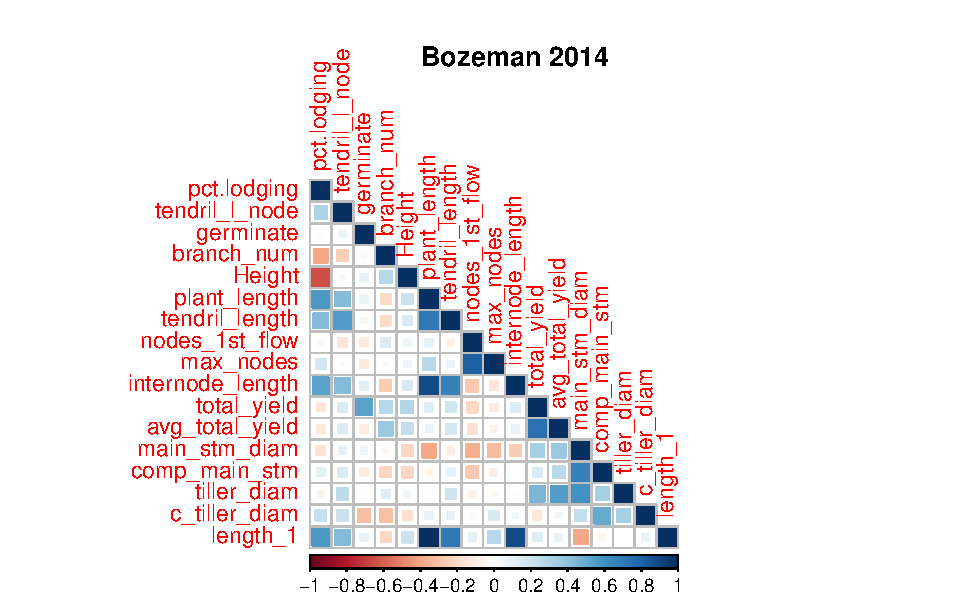
\includegraphics[width=\maxwidth]{figure/nextchunk-1} 

}




{\centering 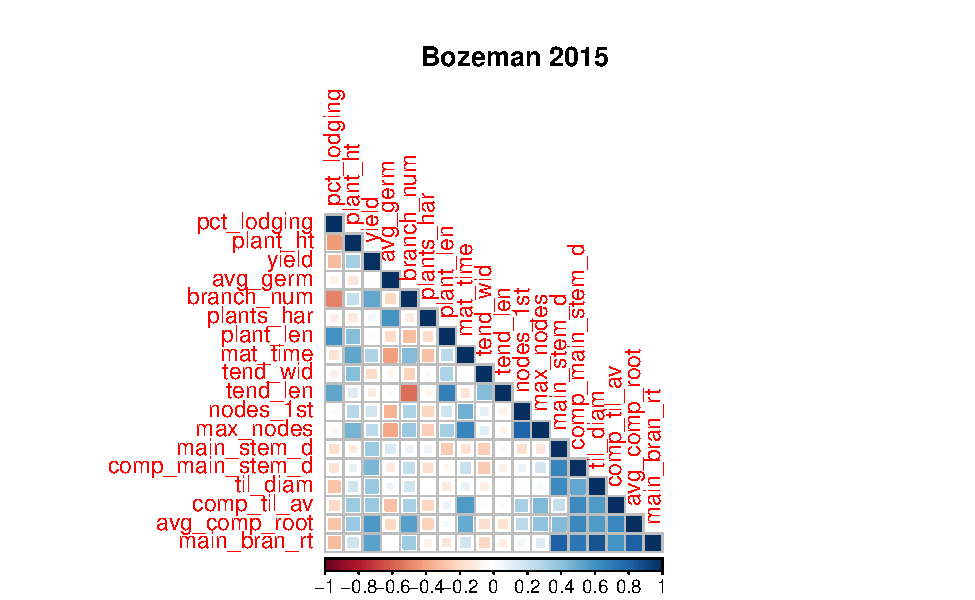
\includegraphics[width=\maxwidth]{figure/nextchunk-2} 

}



\end{knitrout}

\subsection{Moccasin by Year}
Examining the phenotypes at Moccasin in each year, we can see that several of the variables were relatively highly correlated in 2016. The strongest correlations were between tendril length and plant length, which makes sense, as well as between percent lodging and plant length. While none of the correlations would be interpreted as very strong, there are moderate postive and negative relationships in both years. 



\begin{knitrout}\footnotesize
\definecolor{shadecolor}{rgb}{1, 1, 1}\color{fgcolor}

{\centering 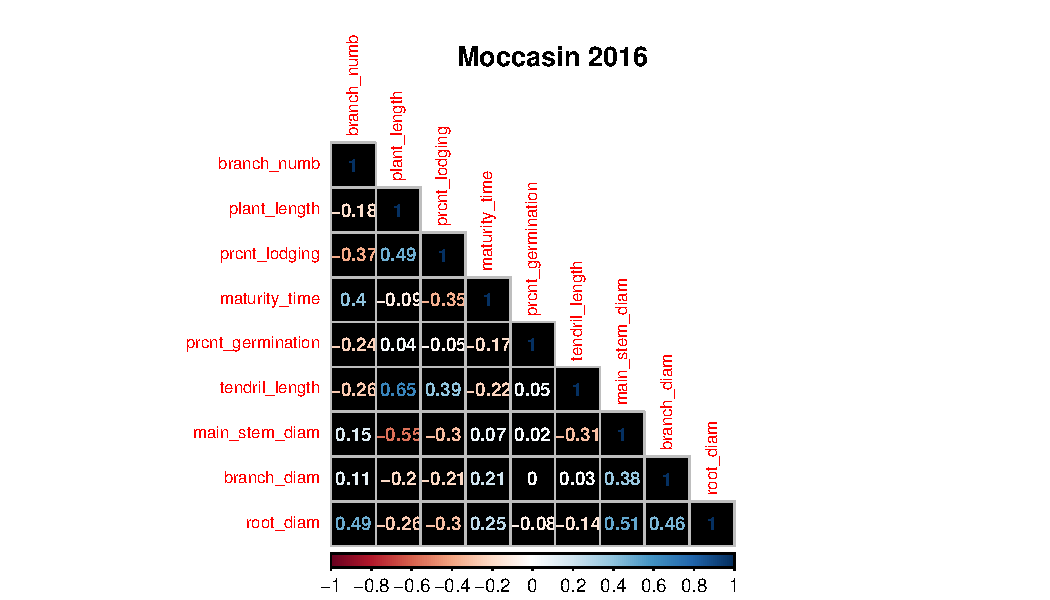
\includegraphics[width=\maxwidth]{figure/moc-1} 

}



\end{knitrout}
\pagebreak
In Moccasin in 2015, several notable correlations were found. Stress minus equation was strongly negatively correlated with tiller diameter, tiller compressed, tiller compressed flex, and flex after crushing. Lodging was not found to be moderately correlated with plant height as expected. 

\begin{knitrout}\footnotesize
\definecolor{shadecolor}{rgb}{1, 1, 1}\color{fgcolor}

{\centering 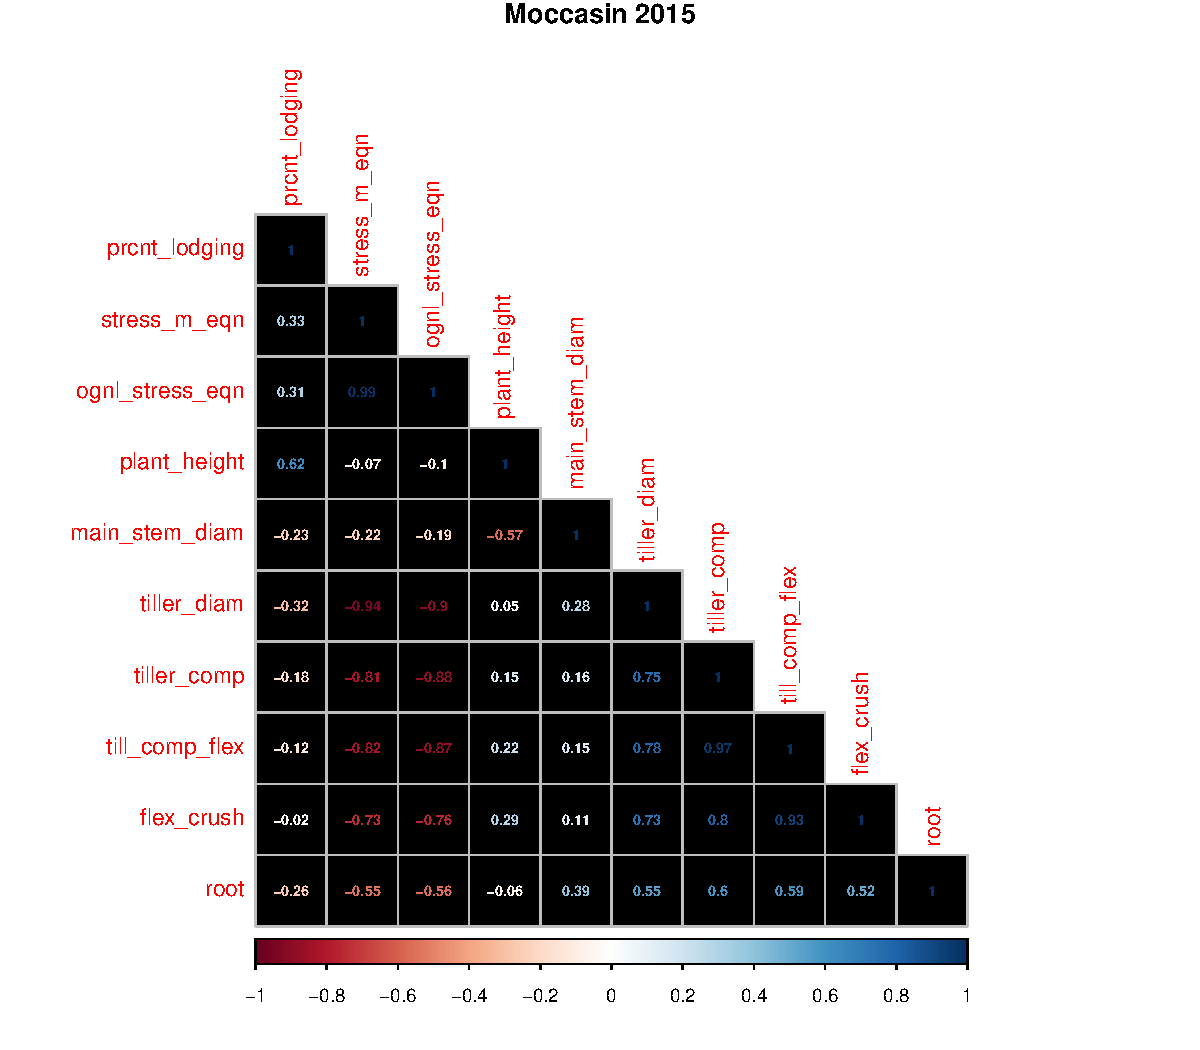
\includegraphics[width=\maxwidth]{figure/Moc15-1} 

}




{\centering 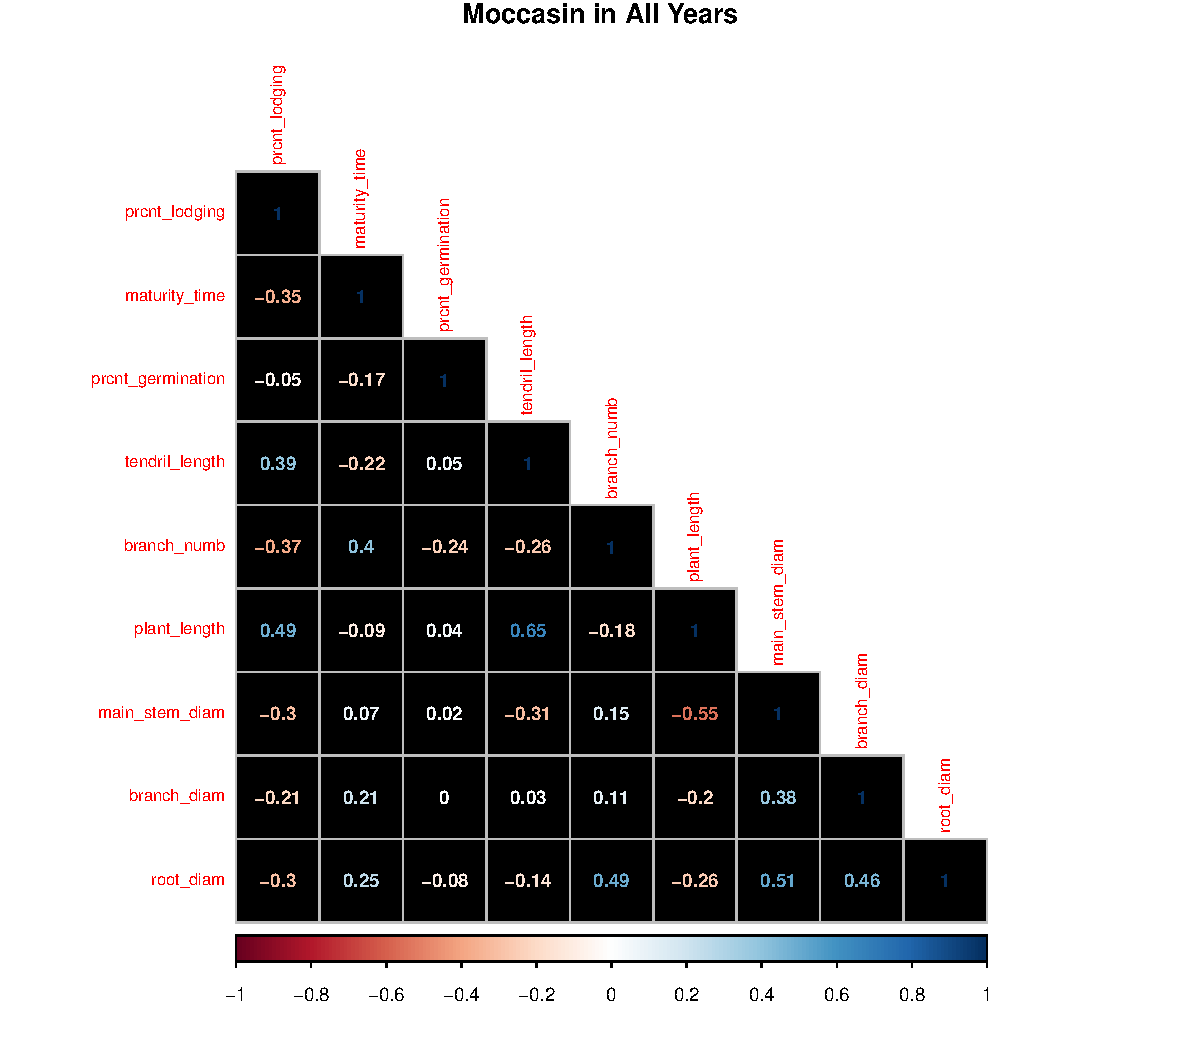
\includegraphics[width=\maxwidth]{figure/Moc15-2} 

}



\end{knitrout}
\pagebreak

\section{Site Year Combinations for Lodging}




\subsection{Exploratory Analysis} 
The data were collected over a period of 4 field seasons at sites in Bozeman and 2 field seasons in Moccasin. Phenotypic data were analyzed in order to determine whether conditions were similar enough at each year/site combination to consider as a single dataset, or if they differ by enough that the sites and years need to be considered as different groups.  

Though QTL analyses of all phenotypic traits is of interest, lodging is considered the primary response. Therefore, we examine the Percent Lodging measured at each site/year combination. Note that Percent Lodging is not measured in the 2013 Bozeman data; we did not include it in this analysis.

Visually, we can create beanplots to assess the differences mean percent lodging at each year/site combination.  These show both the variability of the distribution, like a traditional boxplot would, as well as information about the skew and modes. Over all years in Bozeman it appears that the distribution of lodging was slightly more variable than for sites in Moccasin; however, for some reason in 2016 the Bozeman site exhibited positive skew.  This indicates that in 2016, the majority of pea plants were lodged to a lesser degree than in 2015 or 2014.  The horizontal black bars indicate the original data values. 


\begin{knitrout}\footnotesize
\definecolor{shadecolor}{rgb}{1, 1, 1}\color{fgcolor}

{\centering 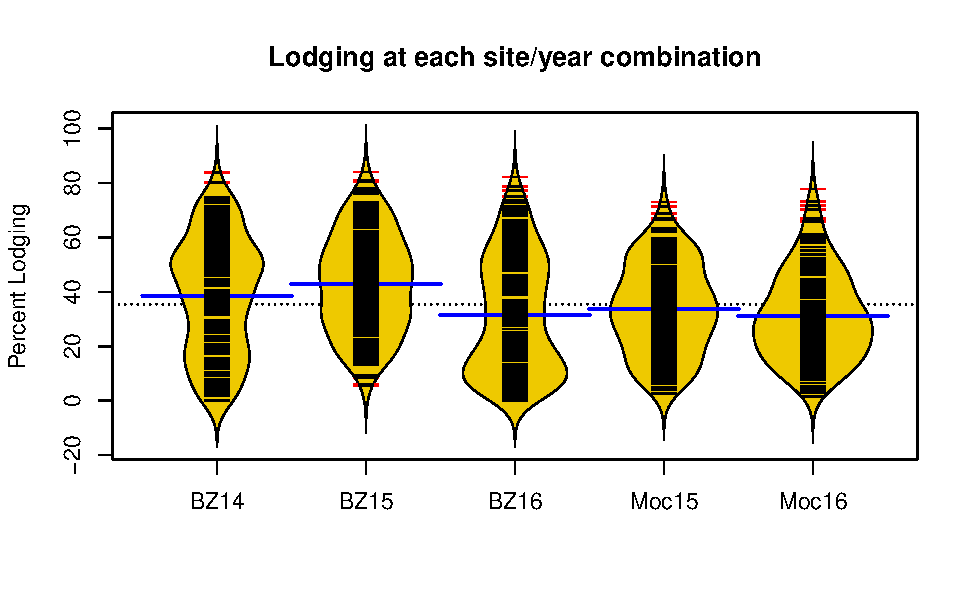
\includegraphics[width=\maxwidth]{figure/meanvars-1} 

}



\end{knitrout}


\subsection{Interaction Plot}
If the sites are reasonably similar, we would expect to see parallel lines that are either overlapping or very near each other.  The red line for Bozeman indicates that average percent lodging was higher in Bozeman than in Moccasin in both 2015 and 2016.  The bars indicate the variability of lodging for each year in Bozeman - it appears that for most years, Bozeman was slightly more variable than Moccasin. While the blue line and red line are both decreasing from 2015 to 2016, the difference in slopes indicates that there may be some interaction between year/site combinations.  More formal testing is necessary to assess differences between year and site combinations, but this visualization indicates some evidence of a difference in lodging in each location and year.
\begin{knitrout}\footnotesize
\definecolor{shadecolor}{rgb}{1, 1, 1}\color{fgcolor}

{\centering 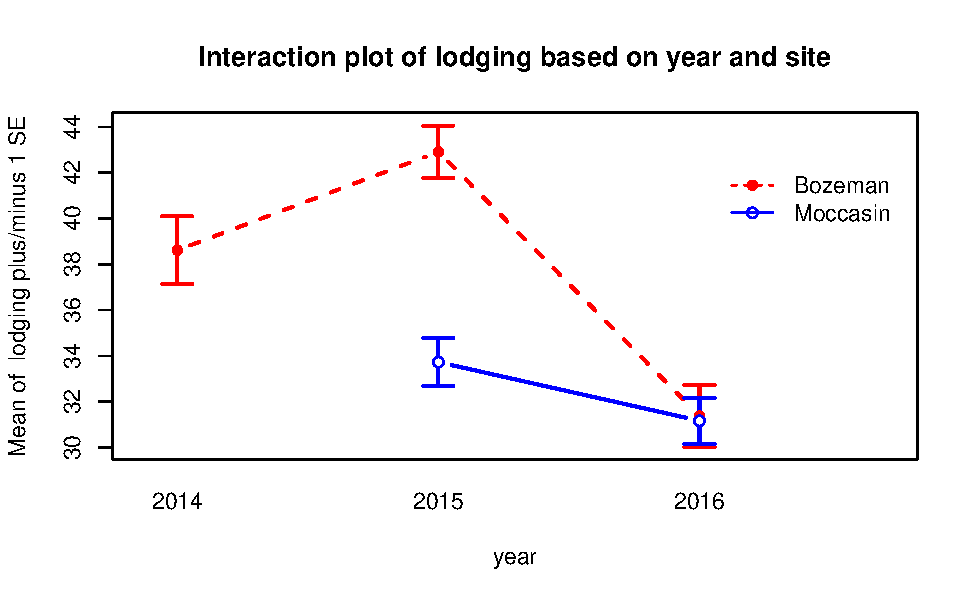
\includegraphics[width=\maxwidth]{figure/tables-1} 

}



\end{knitrout}

\pagebreak
\subsection{Regression Model and Pairwise Comparisons}
Bozeman 2014 was treated as the baseline group. An overall F test using 4 and 1205 degrees of freedom to assess evidence against all site-year combinations yields a p-value less than 0.000001. There is strong evidence that the site/year combinations are not all the same. 
  
We include 95 percent confidence intervals for the true mean percent lodging at each site-year combination. In order to get a better sense for which groups differ, we performed Tukey-Kramer pairwise comparisons to adjust for multiple testing. The results of that analysis are included below. The plot below shows differing pairwise combinations were between Bozeman 2015 and Bozeman 2014, as well as between Moccasin 2015 and Bozeman 2016, and between Moccasin 2016 with Bozeman in 2015 and 2016. Given that Bozeman 2015 had such a large mean relative to the other site/year combinations, this is not a surprising result. 
  
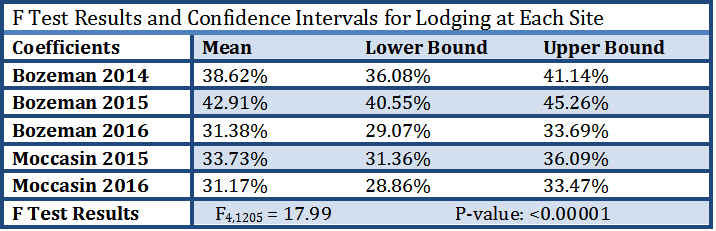
\includegraphics [width = 4.5 in] {RegressionResults}


\begin{knitrout}\footnotesize
\definecolor{shadecolor}{rgb}{1, 1, 1}\color{fgcolor}

{\centering 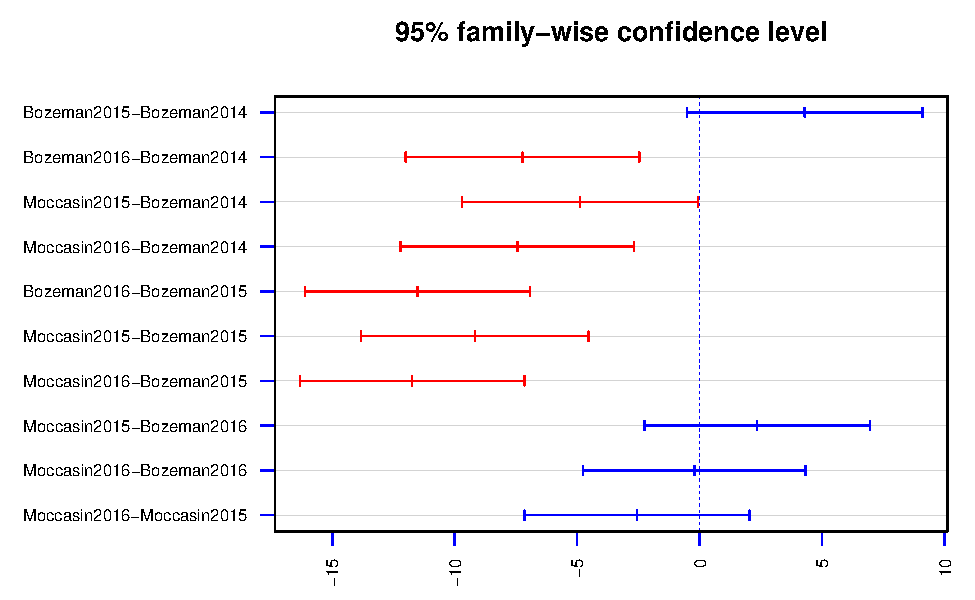
\includegraphics[width=\maxwidth]{figure/tukey-1} 

}



\end{knitrout}


\subsection{Discussion}
This analysis indicates that the measurements taken at each site in each year should be treated separately; they should not be considered homogeneous enough to be taken as a single group.  The inclusion of 2013 into the data is unlikely to change the results of this study because the differences between the combinations already considered are enough to justify splitting the dataset into separate groups.  However, it may facilitate future calculations to consider converting lodging measurements in Bozeman in 2013 from likert-scale format (on a 1-4 scale) to the same "percent-lodging" variable that is used in subsequent years. 


\pagebreak
\section{Missing Genetic Data}
Quality of the genetic data can be explored through the percentage of varieties missing information at each genetic marker. Reviewing QTL literature may provide insight to acceptable missing rates. Plots are provided below to visualize the amount of missing data at each genetic marker and across each variety genotyped. Tables of missing rates are provided in the appendix. As the number of genetic markers and varieties are large, the tables will be more informative on the exact varieties with certain missing rates. Rates of missing-ness at each genetic marker are first shown across all makers, and then are broken in to plots subsetted by genetic markers with less than 25\% missing, less than between 25\% and 30\% missing, less than between 30\% and 35\% missing, and less than between 35\% and 40\%. All genetic markers had at least 60\% of the data across all varieties.

\subsection{All Markers}

\begin{knitrout}\footnotesize
\definecolor{shadecolor}{rgb}{1, 1, 1}\color{fgcolor}\begin{figure}[H]

{\centering 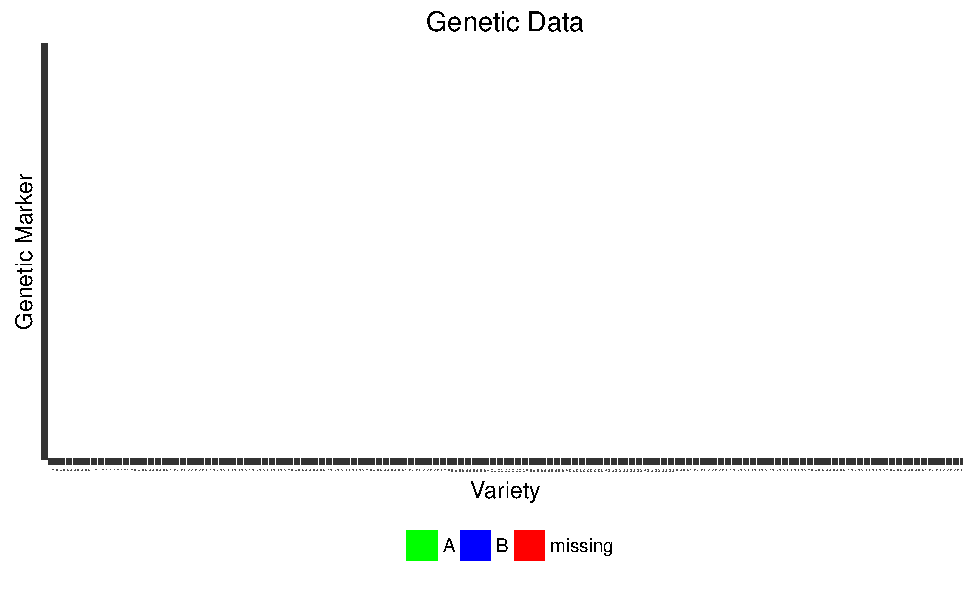
\includegraphics[width=\maxwidth]{figure/missing_plot-1} 

}

\caption[Missing Genetic Data Plot]{Missing Genetic Data Plot}\label{fig:missing.plot}
\end{figure}


\end{knitrout}


\pagebreak

\subsection{Less than 25\% Missing}




\begin{knitrout}\footnotesize
\definecolor{shadecolor}{rgb}{1, 1, 1}\color{fgcolor}

{\centering 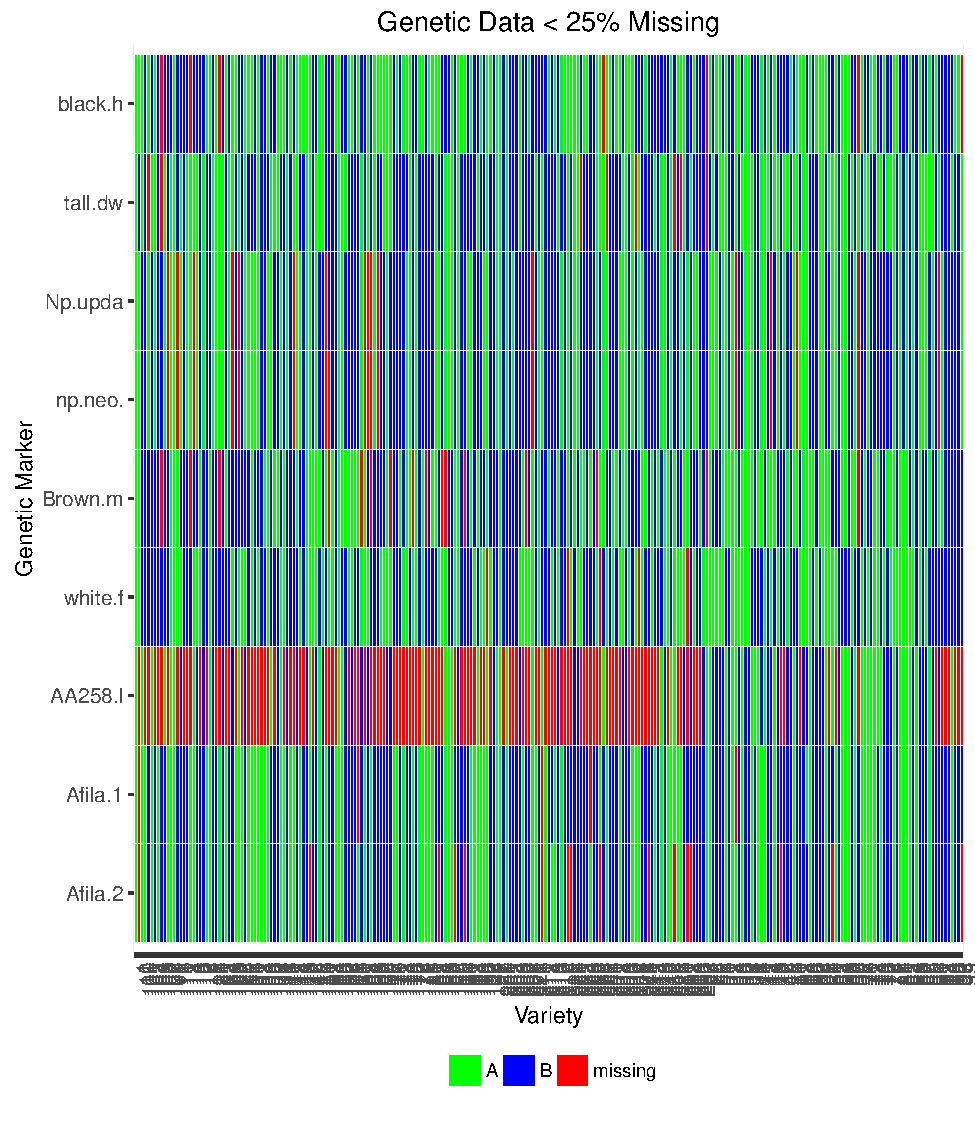
\includegraphics[width=\maxwidth]{figure/missing_plot25-1} 

}



\end{knitrout}
\pagebreak
\subsection{25\% - 30\% Missing}

\begin{knitrout}\footnotesize
\definecolor{shadecolor}{rgb}{1, 1, 1}\color{fgcolor}

{\centering 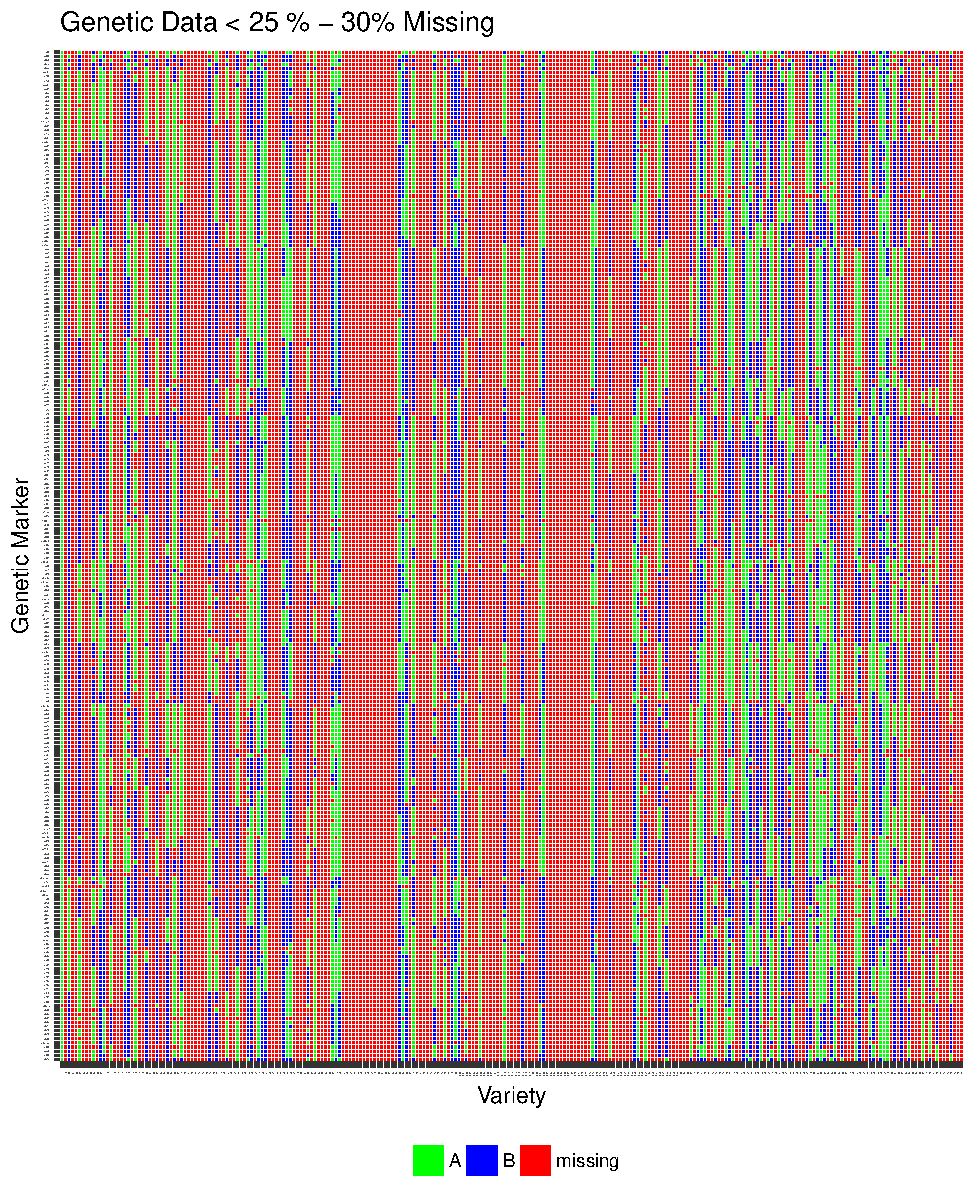
\includegraphics[width=\maxwidth]{figure/missing_plot30-1} 

}



\end{knitrout}
\pagebreak
\subsection{30\% - 35\% Missing}


\begin{knitrout}\footnotesize
\definecolor{shadecolor}{rgb}{1, 1, 1}\color{fgcolor}

{\centering 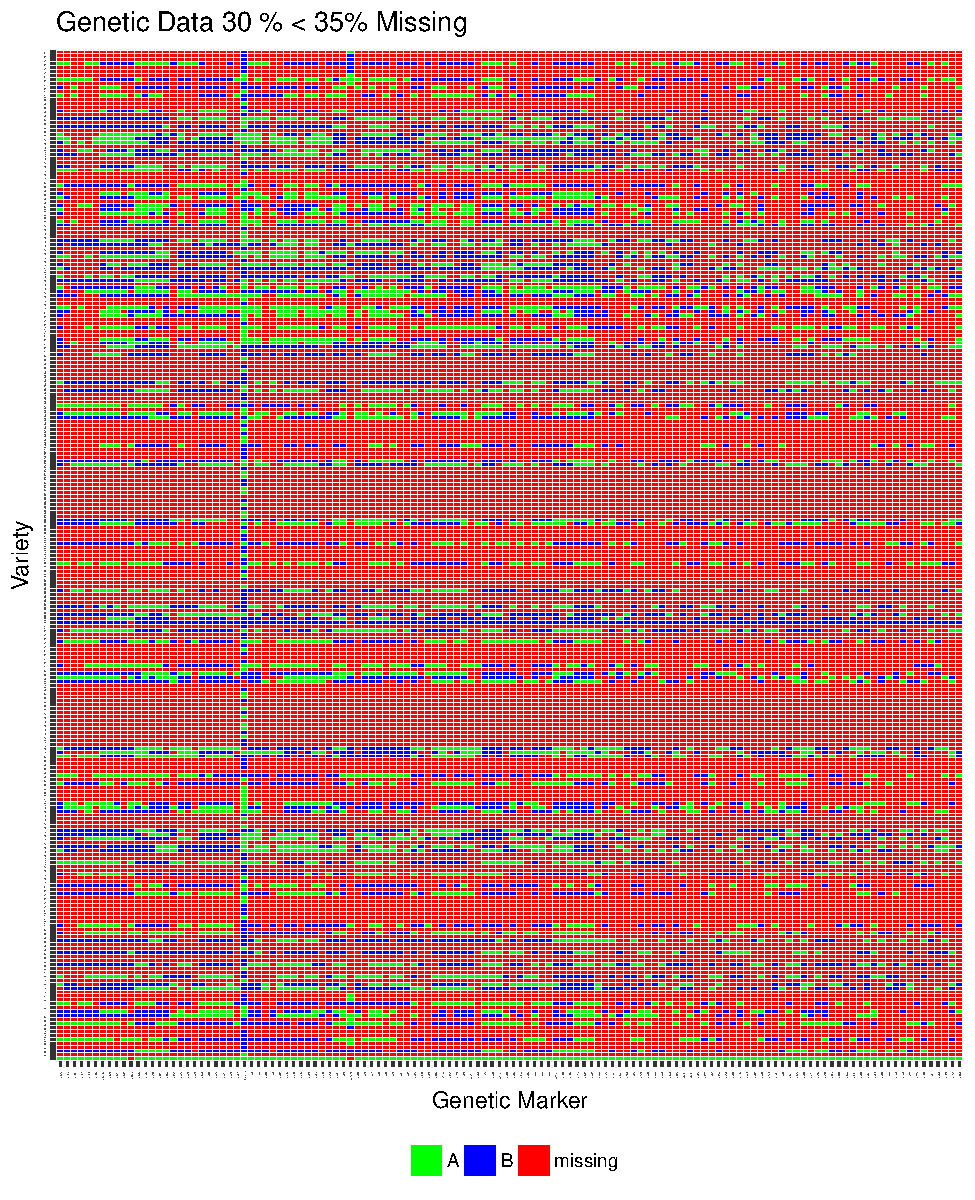
\includegraphics[width=\maxwidth]{figure/missing_plot35-1} 

}



\end{knitrout}
\pagebreak
\subsection{35\% - 40\% Missing}


\begin{knitrout}\footnotesize
\definecolor{shadecolor}{rgb}{1, 1, 1}\color{fgcolor}

{\centering 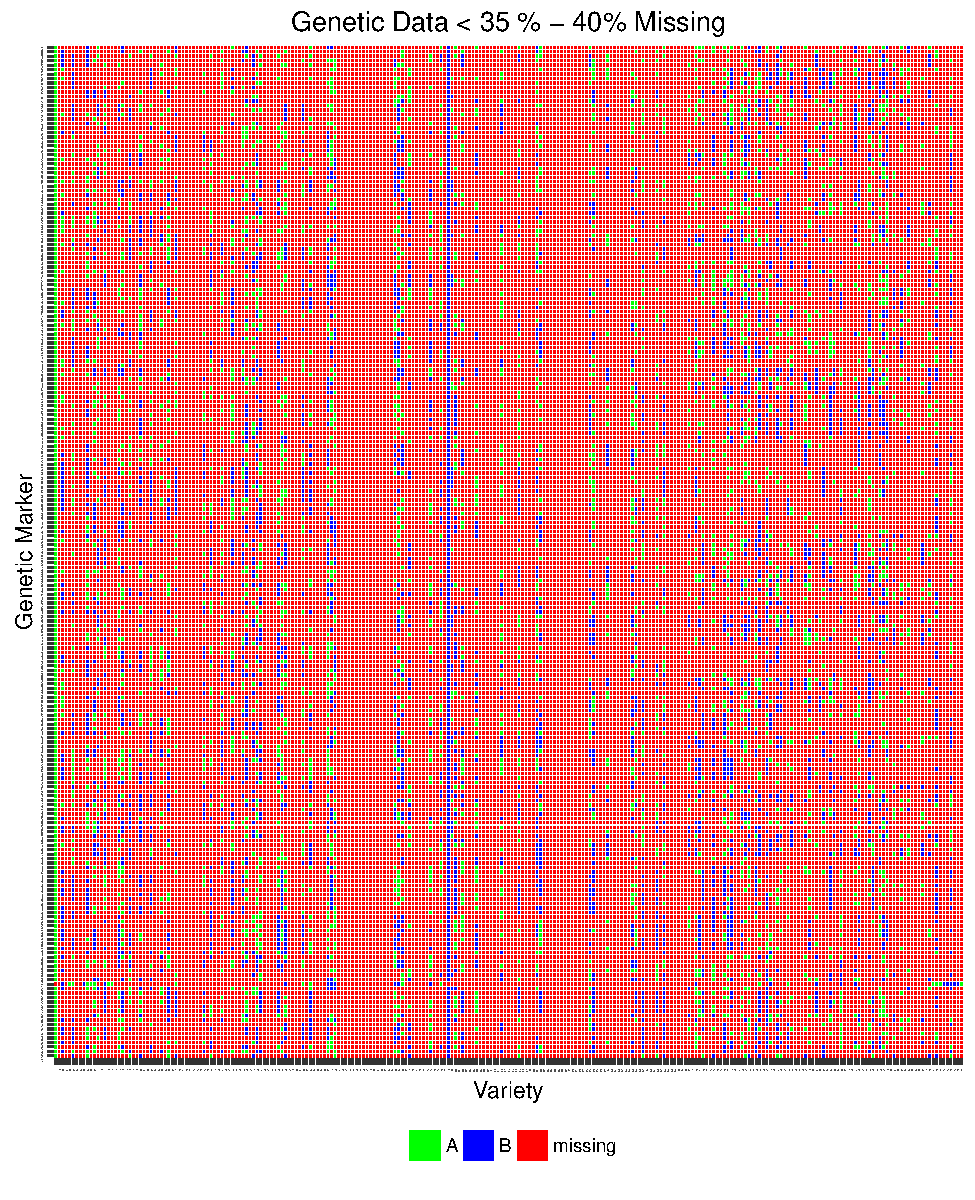
\includegraphics[width=\maxwidth]{figure/missing_plot40-1} 

}



\end{knitrout}












\section{Setting Significance Thresholds}

The pea genetic data include over 600 genetic markers. When a QTL analysis is done, a significance test is done at each marker. Multiple testing problems are quite common in genetic analyses. Jamin mentioned he would like to use LOD for setting a significance threshold. LOD is an abbreviation for the log-odds. LOD is the $log_{10}$ likelihood ratio comparing the null that there is not a QTL to the alternative, that there is.

Null Model, $H_{o}: y_{i} \sim N(\mu, \sigma^2)$ i.e. there is no genetic dependency between the phenotype and the genotype

- Where the maximum likelihood estimates (MLEs) for parameter estimates $\mu = \bar{y}; \sigma^2 = RSS_{o}/n$ are used.

Alternative Model, $H_{a}: y_{i}|g_{i} \sim N(\mu_{g_{i}}, \sigma^2)$

- Where $g_{i}$ = genotype of individual i at the marker (loci); each genotype group has a different mean; $\sigma^2$ = pooled RSS = $RSS_{1}$; again the MLEs. 

LOD = $\frac{n}{2} \times log_{10}(\frac{RSS_{o}}{RSS_{1}})$

LOD is related to the F statistic. LOD = $\frac{n}{2} \times [F({\frac{df}{n-df-1} + 1)]$ and similar to the F statistic, large LOD values are associated with strong evidence for the alternative, that there is a relationship to the genetic loci and the phenotype. Since F statistics help find p-values, and LOD is related to F statistics, by setting genome wide adjusted LOD thresholds, we can easily convert these back to genome wide adjusted p-values. Broman and Sen (2009) provide a simulation based method for generating genome wide adjusted LOD thresholds, and the corresponding genome-wide adjusted p-value thresholds in Section 4.3 using the {\texttt QTL} package in R. 

\section{Future Work}

Future work with Jamin should be more focused with the QTL analysis and developing p-value based thresholds for significance. Jamin currently is using the MapDisto macro in Excel and QTL Cartographer to do preliminary QTL analyses. Both programs provide extensive documentation on their functions. R is a common program for statisticians to use, and discussion around whether packages such as {\texttt QTL} in R or outside programs should be used in the final analysis would be beneficial. While identifying specific genetic markers associated with the most variation in phenotypic traits is the end goal of the project, a QTL analysis has many steps that should be taken before using outputted results. Broman and Sen (2009) is a good reference for a basic QTL analysis. Because Jamin is interested in genetic variation associated with all phenotypic traits, the correlations between the traits should be accounted for in the final analysis. Adding in the recommendation to not combine across sites and years, we suggest the direction of the final QTL analysis done to be in a multi-trait, multi-environment setting. A resource for an introduction to the multi-trait, multi-environment setting in QTL analyses is referenced by Margarido et al. (2015).

\newpage
\section*{References}
\setlength{\parindent}{-0.2in}
\setlength{\leftskip}{0.2in}
\setlength{\parskip}{3pt}
\noindent

Margarido et al. 2015. {\it Multi-trait multi-environment quantitative trait loci mapping for a sugarcane commercial cross provides insights on the inheritance of important traits}. Mol Breeding 35:175.

Broman and Sen. 2009. {\it A guide to QTL mapping with R/QTL}. New York: Spring Science+Business Media. Retrieved from 

\url{http://link.springer.com/book/10.1007%2F978-0-387-92125-9}.

\setlength{\parindent}{0in}
\setlength{\leftskip}{0in}
\setlength{\parskip}{8pt}

\newpage


\section*{Appendix}
{\bf Tables of Missing Rates by Genetic Marker}

% latex table generated in R 3.3.2 by xtable 1.8-2 package
% Thu Dec 15 23:21:49 2016
\begin{table}[H]
\centering
\scalebox{0.5}{
\begin{tabular}{rrrrrrrrrrrrrrrrrrrrr}
  \hline
 & A1617 & A1621 & A1619 & A1618 & A1624 & A1615 & A1622 & A7578 & C20B & AD51.ba & A6734 & A6726 & A6730 & A6732 & A6733 & A6731 & A6737 & A6724 & A6729 & A6738 \\ 
  \hline
Count & 194.00 & 199.00 & 202.00 & 195.00 & 199.00 & 185.00 & 163.00 & 163.00 & 170.00 & 166.00 & 209.00 & 162.00 & 161.00 & 161.00 & 210.00 & 166.00 & 190.00 & 163.00 & 182.00 & 193.00 \\ 
  Percent & 0.32 & 0.33 & 0.33 & 0.32 & 0.33 & 0.30 & 0.27 & 0.27 & 0.28 & 0.27 & 0.34 & 0.27 & 0.26 & 0.26 & 0.34 & 0.27 & 0.31 & 0.27 & 0.30 & 0.32 \\ 
   \hline
\end{tabular}
}
\end{table}
% latex table generated in R 3.3.2 by xtable 1.8-2 package
% Thu Dec 15 23:21:49 2016
\begin{table}[H]
\centering
\scalebox{0.5}{
\begin{tabular}{rrrrrrrrrrrrrrrrrrrrr}
  \hline
 & A6725 & A6728 & A004..s & A1623 & A1620 & A1303 & A1616 & A1331 & A1325 & A1327 & A1329 & A1330 & A1332 & A1409 & A1408 & A2407 & A1405 & A1404 & A1402 & A1403 \\ 
  \hline
Count & 163.00 & 165.00 & 173.00 & 185.00 & 162.00 & 161.00 & 168.00 & 164.00 & 161.00 & 161.00 & 161.00 & 161.00 & 161.00 & 161.00 & 161.00 & 161.00 & 187.00 & 169.00 & 193.00 & 176.00 \\ 
  Percent & 0.27 & 0.27 & 0.28 & 0.30 & 0.27 & 0.26 & 0.28 & 0.27 & 0.26 & 0.26 & 0.26 & 0.26 & 0.26 & 0.26 & 0.26 & 0.26 & 0.31 & 0.28 & 0.32 & 0.29 \\ 
   \hline
\end{tabular}
}
\end{table}
% latex table generated in R 3.3.2 by xtable 1.8-2 package
% Thu Dec 15 23:21:49 2016
\begin{table}[H]
\centering
\scalebox{0.5}{
\begin{tabular}{rrrrrrrrrrrrrrrrrrrrr}
  \hline
 & A1024 & ad147.l & A7384 & A7380 & A7302 & A7302.1 & A2197 & A6889 & A6891 & A2259 & A2257 & A2256 & A2521 & A5967 & A2340 & A26 & A26.dpn & A26.dpn.1 & Ab56..D & Afila.2 \\ 
  \hline
Count & 162.00 & 163.00 & 162.00 & 163.00 & 163.00 & 211.00 & 226.00 & 164.00 & 163.00 & 187.00 & 170.00 & 201.00 & 161.00 & 162.00 & 162.00 & 161.00 & 165.00 & 165.00 & 182.00 & 16.00 \\ 
  Percent & 0.27 & 0.27 & 0.27 & 0.27 & 0.27 & 0.35 & 0.37 & 0.27 & 0.27 & 0.31 & 0.28 & 0.33 & 0.26 & 0.27 & 0.27 & 0.26 & 0.27 & 0.27 & 0.30 & 0.03 \\ 
   \hline
\end{tabular}
}
\end{table}
% latex table generated in R 3.3.2 by xtable 1.8-2 package
% Thu Dec 15 23:21:49 2016
\begin{table}[H]
\centering
\scalebox{0.5}{
\begin{tabular}{rrrrrrrrrrrrrrrrrrrrr}
  \hline
 & Afila.l & Afila.1 & AA258.l & AD51.ba.1 & A6953 & A5189 & A6757 & A6755 & A6648 & AA473.L & A6762 & A6758 & AA332.L & A4834 & A4832 & AA5.Mid & AA372.L & white.f & white.f.1 & A6085 \\ 
  \hline
Count & 163.00 & 5.00 & 129.00 & 166.00 & 218.00 & 192.00 & 171.00 & 161.00 & 161.00 & 164.00 & 162.00 & 162.00 & 162.00 & 161.00 & 163.00 & 171.00 & 166.00 & 5.00 & 161.00 & 163.00 \\ 
  Percent & 0.27 & 0.01 & 0.21 & 0.27 & 0.36 & 0.32 & 0.28 & 0.26 & 0.26 & 0.27 & 0.27 & 0.27 & 0.27 & 0.26 & 0.27 & 0.28 & 0.27 & 0.01 & 0.26 & 0.27 \\ 
   \hline
\end{tabular}
}
\end{table}
% latex table generated in R 3.3.2 by xtable 1.8-2 package
% Thu Dec 15 23:21:49 2016
\begin{table}[H]
\centering
\scalebox{0.5}{
\begin{tabular}{rrrrrrrrrrrrrrrrrrrrr}
  \hline
 & A6086 & A6087 & A854 & A853 & A4507 & A4500 & A337 & A4495 & A4496 & A7738 & A7732 & A4497 & A298 & A7055 & A4292 & A6470 & A5495 & A5502 & A220 & A5501 \\ 
  \hline
Count & 167.00 & 163.00 & 162.00 & 162.00 & 171.00 & 163.00 & 172.00 & 173.00 & 195.00 & 208.00 & 215.00 & 205.00 & 162.00 & 169.00 & 161.00 & 162.00 & 199.00 & 166.00 & 171.00 & 184.00 \\ 
  Percent & 0.27 & 0.27 & 0.27 & 0.27 & 0.28 & 0.27 & 0.28 & 0.28 & 0.32 & 0.34 & 0.35 & 0.34 & 0.27 & 0.28 & 0.26 & 0.27 & 0.33 & 0.27 & 0.28 & 0.30 \\ 
   \hline
\end{tabular}
}
\end{table}
% latex table generated in R 3.3.2 by xtable 1.8-2 package
% Thu Dec 15 23:21:50 2016
\begin{table}[H]
\centering
\scalebox{0.5}{
\begin{tabular}{rrrrrrrrrrrrrrrrrrrrr}
  \hline
 & A5494 & A5499 & A5491 & A5498 & A299 & A1561 & A7736 & A4494 & A4508 & A4502 & A4501 & A7729 & A7734 & A7733 & A4499 & A7740 & A7258 & A7257 & AD51.Ba & A5204 \\ 
  \hline
Count & 166.00 & 190.00 & 169.00 & 198.00 & 202.00 & 181.00 & 180.00 & 163.00 & 162.00 & 162.00 & 161.00 & 166.00 & 165.00 & 161.00 & 219.00 & 163.00 & 164.00 & 167.00 & 171.00 & 223.00 \\ 
  Percent & 0.27 & 0.31 & 0.28 & 0.33 & 0.33 & 0.30 & 0.30 & 0.27 & 0.27 & 0.27 & 0.26 & 0.27 & 0.27 & 0.26 & 0.36 & 0.27 & 0.27 & 0.27 & 0.28 & 0.37 \\ 
   \hline
\end{tabular}
}
\end{table}
% latex table generated in R 3.3.2 by xtable 1.8-2 package
% Thu Dec 15 23:21:50 2016
\begin{table}[H]
\centering
\scalebox{0.5}{
\begin{tabular}{rrrrrrrrrrrrrrrrrrrrr}
  \hline
 & A5213 & A5165 & A5193 & A5191 & Brown.m & A60 & A56 & A61 & A55 & A57 & A59 & A5226 & A58 & A5229 & LKA.F5. & A7184 & A7183 & A7181 & A7185 & A7182 \\ 
  \hline
Count & 224.00 & 206.00 & 217.00 & 227.00 & 16.00 & 190.00 & 182.00 & 190.00 & 168.00 & 165.00 & 193.00 & 220.00 & 208.00 & 189.00 & 186.00 & 162.00 & 192.00 & 164.00 & 164.00 & 163.00 \\ 
  Percent & 0.37 & 0.34 & 0.36 & 0.37 & 0.03 & 0.31 & 0.30 & 0.31 & 0.28 & 0.27 & 0.32 & 0.36 & 0.34 & 0.31 & 0.31 & 0.27 & 0.32 & 0.27 & 0.27 & 0.27 \\ 
   \hline
\end{tabular}
}
\end{table}
% latex table generated in R 3.3.2 by xtable 1.8-2 package
% Thu Dec 15 23:21:50 2016
\begin{table}[H]
\centering
\scalebox{0.5}{
\begin{tabular}{rrrrrrrrrrrrrrrrrrrrr}
  \hline
 & A2446 & A7188 & A7186 & A7187 & A7356 & A7357 & A7298 & A4307 & AA107.. & A6492 & A7814 & A7814.1 & A5160 & A7346 & A7339 & A7371 & A7340 & A7359 & A7369 & A7348 \\ 
  \hline
Count & 162.00 & 161.00 & 169.00 & 200.00 & 207.00 & 178.00 & 166.00 & 196.00 & 164.00 & 163.00 & 161.00 & 191.00 & 216.00 & 196.00 & 213.00 & 220.00 & 216.00 & 216.00 & 217.00 & 217.00 \\ 
  Percent & 0.27 & 0.26 & 0.28 & 0.33 & 0.34 & 0.29 & 0.27 & 0.32 & 0.27 & 0.27 & 0.26 & 0.31 & 0.35 & 0.32 & 0.35 & 0.36 & 0.35 & 0.35 & 0.36 & 0.36 \\ 
   \hline
\end{tabular}
}
\end{table}
% latex table generated in R 3.3.2 by xtable 1.8-2 package
% Thu Dec 15 23:21:50 2016
\begin{table}[H]
\centering
\scalebox{0.5}{
\begin{tabular}{rrrrrrrrrrrrrrrrrrrrr}
  \hline
 & A2431 & A6253 & A6252 & A6254 & A6622 & A4829 & AD73.f. & AB111.L & A6075 & A6995 & A4460 & AA5..Lo & A4461 & A6994 & A2246 & A1025 & AD174.L & CDC.27. & A836 & A836.1 \\ 
  \hline
Count & 218.00 & 164.00 & 164.00 & 162.00 & 163.00 & 164.00 & 164.00 & 162.00 & 163.00 & 181.00 & 162.00 & 162.00 & 165.00 & 199.00 & 169.00 & 162.00 & 164.00 & 170.00 & 161.00 & 213.00 \\ 
  Percent & 0.36 & 0.27 & 0.27 & 0.27 & 0.27 & 0.27 & 0.27 & 0.27 & 0.27 & 0.30 & 0.27 & 0.27 & 0.27 & 0.33 & 0.28 & 0.27 & 0.27 & 0.28 & 0.26 & 0.35 \\ 
   \hline
\end{tabular}
}
\end{table}
% latex table generated in R 3.3.2 by xtable 1.8-2 package
% Thu Dec 15 23:21:50 2016
\begin{table}[H]
\centering
\scalebox{0.5}{
\begin{tabular}{rrrrrrrrrrrrrrrrrrrrr}
  \hline
 & NCPA.F2 & A5200 & A430 & A420 & A413 & A145 & A422 & A428 & A432 & A421 & A423 & A425 & np.neo. & Np.upda & AD270.L & tall.dw & A1063 & A1066 & A1064 & A1065 \\ 
  \hline
Count & 219.00 & 198.00 & 186.00 & 200.00 & 166.00 & 201.00 & 163.00 & 203.00 & 184.00 & 189.00 & 207.00 & 186.00 & 18.00 & 17.00 & 169.00 & 8.00 & 161.00 & 163.00 & 162.00 & 179.00 \\ 
  Percent & 0.36 & 0.33 & 0.31 & 0.33 & 0.27 & 0.33 & 0.27 & 0.33 & 0.30 & 0.31 & 0.34 & 0.31 & 0.03 & 0.03 & 0.28 & 0.01 & 0.26 & 0.27 & 0.27 & 0.29 \\ 
   \hline
\end{tabular}
}
\end{table}
% latex table generated in R 3.3.2 by xtable 1.8-2 package
% Thu Dec 15 23:21:50 2016
\begin{table}[H]
\centering
\scalebox{0.5}{
\begin{tabular}{rrrrrrrrrrrrrrrrrrrrr}
  \hline
 & AA285.D & A6802 & A6800 & A6801 & A6160 & P628.Hi & A7837 & A2100 & A5640 & A783 & A5896 & A2004 & A2342 & A9.lg.4 & A2343 & A1996 & A2002 & A2006 & A1221 & A1224 \\ 
  \hline
Count & 164.00 & 162.00 & 162.00 & 166.00 & 162.00 & 182.00 & 171.00 & 200.00 & 206.00 & 220.00 & 226.00 & 187.00 & 208.00 & 162.00 & 202.00 & 183.00 & 190.00 & 163.00 & 164.00 & 166.00 \\ 
  Percent & 0.27 & 0.27 & 0.27 & 0.27 & 0.27 & 0.30 & 0.28 & 0.33 & 0.34 & 0.36 & 0.37 & 0.31 & 0.34 & 0.27 & 0.33 & 0.30 & 0.31 & 0.27 & 0.27 & 0.27 \\ 
   \hline
\end{tabular}
}
\end{table}
% latex table generated in R 3.3.2 by xtable 1.8-2 package
% Thu Dec 15 23:21:50 2016
\begin{table}[H]
\centering
\scalebox{0.5}{
\begin{tabular}{rrrrrrrrrrrrrrrrrrrrr}
  \hline
 & A2012 & A2008 & A1223 & A2007 & A2341 & A2001 & A7189 & A7192 & A7193 & A7197 & A7196 & A296 & AGAT.Hi & A2181 & A4598 & A7749 & A4852 & A6542 & A1785 & A1788 \\ 
  \hline
Count & 176.00 & 162.00 & 163.00 & 163.00 & 162.00 & 161.00 & 161.00 & 163.00 & 163.00 & 164.00 & 168.00 & 162.00 & 185.00 & 185.00 & 162.00 & 162.00 & 228.00 & 194.00 & 161.00 & 161.00 \\ 
  Percent & 0.29 & 0.27 & 0.27 & 0.27 & 0.27 & 0.26 & 0.26 & 0.27 & 0.27 & 0.27 & 0.28 & 0.27 & 0.30 & 0.30 & 0.27 & 0.27 & 0.37 & 0.32 & 0.26 & 0.26 \\ 
   \hline
\end{tabular}
}
\end{table}
% latex table generated in R 3.3.2 by xtable 1.8-2 package
% Thu Dec 15 23:21:50 2016
\begin{table}[H]
\centering
\scalebox{0.5}{
\begin{tabular}{rrrrrrrrrrrrrrrrrrrrr}
  \hline
 & A1783 & A1787 & A1782 & A1786 & A30 & A37 & A5406 & A5399 & A5402 & A5404 & A5400 & A5398 & AA315.L & A5517 & A4825 & A4826 & A4824 & AB23.lg & AA81 & A4808 \\ 
  \hline
Count & 161.00 & 161.00 & 169.00 & 167.00 & 164.00 & 161.00 & 183.00 & 167.00 & 166.00 & 169.00 & 165.00 & 194.00 & 163.00 & 183.00 & 227.00 & 227.00 & 205.00 & 161.00 & 165.00 & 161.00 \\ 
  Percent & 0.26 & 0.26 & 0.28 & 0.27 & 0.27 & 0.26 & 0.30 & 0.27 & 0.27 & 0.28 & 0.27 & 0.32 & 0.27 & 0.30 & 0.37 & 0.37 & 0.34 & 0.26 & 0.27 & 0.26 \\ 
   \hline
\end{tabular}
}
\end{table}
% latex table generated in R 3.3.2 by xtable 1.8-2 package
% Thu Dec 15 23:21:50 2016
\begin{table}[H]
\centering
\scalebox{0.5}{
\begin{tabular}{rrrrrrrrrrrrrrrrrrrrr}
  \hline
 & A4804 & A4806 & A1822 & A4337 & A4807 & A4809 & A4805 & A1821 & A4827 & A2144 & PYDC.UN & A5227 & A5157 & A7606 & A7611 & A7618 & A7613 & A7621 & A7610 & A7604 \\ 
  \hline
Count & 162.00 & 175.00 & 162.00 & 163.00 & 162.00 & 162.00 & 162.00 & 162.00 & 168.00 & 195.00 & 205.00 & 222.00 & 207.00 & 162.00 & 165.00 & 164.00 & 164.00 & 164.00 & 170.00 & 164.00 \\ 
  Percent & 0.27 & 0.29 & 0.27 & 0.27 & 0.27 & 0.27 & 0.27 & 0.27 & 0.28 & 0.32 & 0.34 & 0.36 & 0.34 & 0.27 & 0.27 & 0.27 & 0.27 & 0.27 & 0.28 & 0.27 \\ 
   \hline
\end{tabular}
}
\end{table}
% latex table generated in R 3.3.2 by xtable 1.8-2 package
% Thu Dec 15 23:21:50 2016
\begin{table}[H]
\centering
\scalebox{0.5}{
\begin{tabular}{rrrrrrrrrrrrrrrrrrrrr}
  \hline
 & A7608 & A7607 & A7602 & A7601 & A7615 & A7614 & A7603 & A7619 & A446 & A2518 & A448 & A451 & A452 & A449 & A447 & A445 & A444 & A4546 & AA374.l & AA224.l \\ 
  \hline
Count & 162.00 & 162.00 & 162.00 & 162.00 & 163.00 & 163.00 & 163.00 & 162.00 & 161.00 & 164.00 & 163.00 & 163.00 & 163.00 & 161.00 & 163.00 & 194.00 & 204.00 & 192.00 & 163.00 & 161.00 \\ 
  Percent & 0.27 & 0.27 & 0.27 & 0.27 & 0.27 & 0.27 & 0.27 & 0.27 & 0.26 & 0.27 & 0.27 & 0.27 & 0.27 & 0.26 & 0.27 & 0.32 & 0.33 & 0.32 & 0.27 & 0.26 \\ 
   \hline
\end{tabular}
}
\end{table}
% latex table generated in R 3.3.2 by xtable 1.8-2 package
% Thu Dec 15 23:21:50 2016
\begin{table}[H]
\centering
\scalebox{0.5}{
\begin{tabular}{rrrrrrrrrrrrrrrrrrrrr}
  \hline
 & A7224 & A7223 & A1580 & A5439 & A5420 & A7133 & A7134 & A7132 & A7131 & AA335.L & A1006 & A1004 & A1002 & A1007 & A995 & A996 & A1003 & A1008 & A999 & A998 \\ 
  \hline
Count & 165.00 & 163.00 & 161.00 & 161.00 & 161.00 & 162.00 & 162.00 & 161.00 & 161.00 & 161.00 & 188.00 & 188.00 & 176.00 & 162.00 & 187.00 & 172.00 & 173.00 & 166.00 & 161.00 & 161.00 \\ 
  Percent & 0.27 & 0.27 & 0.26 & 0.26 & 0.26 & 0.27 & 0.27 & 0.26 & 0.26 & 0.26 & 0.31 & 0.31 & 0.29 & 0.27 & 0.31 & 0.28 & 0.28 & 0.27 & 0.26 & 0.26 \\ 
   \hline
\end{tabular}
}
\end{table}
% latex table generated in R 3.3.2 by xtable 1.8-2 package
% Thu Dec 15 23:21:50 2016
\begin{table}[H]
\centering
\scalebox{0.5}{
\begin{tabular}{rrrrrrrrrrrrrrrrrrrrr}
  \hline
 & A997 & A6901 & A1001 & A1000 & A6634 & black.h & A4409 & AC76b.l & A1555 & A6561 & A1915 & A1916 & A6560 & A6563 & A1912 & RPL15S. & A641 & A642 & A649 & A645 \\ 
  \hline
Count & 161.00 & 162.00 & 163.00 & 161.00 & 162.00 & 7.00 & 162.00 & 163.00 & 226.00 & 167.00 & 165.00 & 201.00 & 163.00 & 162.00 & 203.00 & 172.00 & 161.00 & 166.00 & 161.00 & 171.00 \\ 
  Percent & 0.26 & 0.27 & 0.27 & 0.26 & 0.27 & 0.01 & 0.27 & 0.27 & 0.37 & 0.27 & 0.27 & 0.33 & 0.27 & 0.27 & 0.33 & 0.28 & 0.26 & 0.27 & 0.26 & 0.28 \\ 
   \hline
\end{tabular}
}
\end{table}
% latex table generated in R 3.3.2 by xtable 1.8-2 package
% Thu Dec 15 23:21:50 2016
\begin{table}[H]
\centering
\scalebox{0.5}{
\begin{tabular}{rrrrrrrrrrrrrrrrrrrrr}
  \hline
 & A640 & A638 & A647 & A7763 & A4828 & aa456.. & A1978 & A1980 & aa416.. & A258 & A260 & A246 & A66 & A253 & A259 & A236 & A250 & A5553 & A5574 & A5562 \\ 
  \hline
Count & 162.00 & 161.00 & 161.00 & 163.00 & 206.00 & 161.00 & 161.00 & 166.00 & 164.00 & 215.00 & 222.00 & 224.00 & 219.00 & 214.00 & 224.00 & 221.00 & 221.00 & 224.00 & 222.00 & 223.00 \\ 
  Percent & 0.27 & 0.26 & 0.26 & 0.27 & 0.34 & 0.26 & 0.26 & 0.27 & 0.27 & 0.35 & 0.36 & 0.37 & 0.36 & 0.35 & 0.37 & 0.36 & 0.36 & 0.37 & 0.36 & 0.37 \\ 
   \hline
\end{tabular}
}
\end{table}
% latex table generated in R 3.3.2 by xtable 1.8-2 package
% Thu Dec 15 23:21:50 2016
\begin{table}[H]
\centering
\scalebox{0.5}{
\begin{tabular}{rrrrrrrrrrrrrrrrrrrrr}
  \hline
 & A5582 & A5575 & A5567 & A5552 & A5550 & A5545 & A5563 & A5547 & A1434 & A1551 & A6408 & A470 & A474 & A6451 & A6449 & A6454 & A846 & A6751 & A850 & A2680 \\ 
  \hline
Count & 222.00 & 217.00 & 220.00 & 224.00 & 220.00 & 218.00 & 215.00 & 217.00 & 206.00 & 209.00 & 184.00 & 230.00 & 226.00 & 219.00 & 221.00 & 219.00 & 222.00 & 215.00 & 213.00 & 222.00 \\ 
  Percent & 0.36 & 0.36 & 0.36 & 0.37 & 0.36 & 0.36 & 0.35 & 0.36 & 0.34 & 0.34 & 0.30 & 0.38 & 0.37 & 0.36 & 0.36 & 0.36 & 0.36 & 0.35 & 0.35 & 0.36 \\ 
   \hline
\end{tabular}
}
\end{table}
% latex table generated in R 3.3.2 by xtable 1.8-2 package
% Thu Dec 15 23:21:50 2016
\begin{table}[H]
\centering
\scalebox{0.5}{
\begin{tabular}{rrrrrrrrrrrrrrrrrrrrr}
  \hline
 & A3067 & A3050 & A635 & A3598 & A5728 & A5477 & A5478 & A5479 & A6575 & A6049 & A6044 & A6742 & A6297 & A4690 & A791 & A6751.1 & A846.1 & A850.1 & A5311 & A5895 \\ 
  \hline
Count & 220.00 & 217.00 & 205.00 & 199.00 & 211.00 & 208.00 & 209.00 & 206.00 & 171.00 & 214.00 & 219.00 & 220.00 & 198.00 & 206.00 & 220.00 & 215.00 & 222.00 & 213.00 & 192.00 & 223.00 \\ 
  Percent & 0.36 & 0.36 & 0.34 & 0.33 & 0.35 & 0.34 & 0.34 & 0.34 & 0.28 & 0.35 & 0.36 & 0.36 & 0.33 & 0.34 & 0.36 & 0.35 & 0.36 & 0.35 & 0.32 & 0.37 \\ 
   \hline
\end{tabular}
}
\end{table}
% latex table generated in R 3.3.2 by xtable 1.8-2 package
% Thu Dec 15 23:21:50 2016
\begin{table}[H]
\centering
\scalebox{0.5}{
\begin{tabular}{rrrrrrrrrrrrrrrrrrrrr}
  \hline
 & A6329 & A6339 & A1058 & A5537 & A244 & A257 & A232 & A243 & A237 & A240 & A6955 & A6934 & A4750 & A4734 & A4757 & A2714 & A6947 & A938 & A4792 & A4786 \\ 
  \hline
Count & 193.00 & 224.00 & 191.00 & 226.00 & 216.00 & 220.00 & 223.00 & 219.00 & 213.00 & 215.00 & 219.00 & 217.00 & 217.00 & 216.00 & 225.00 & 180.00 & 214.00 & 203.00 & 220.00 & 223.00 \\ 
  Percent & 0.32 & 0.37 & 0.31 & 0.37 & 0.35 & 0.36 & 0.37 & 0.36 & 0.35 & 0.35 & 0.36 & 0.36 & 0.36 & 0.35 & 0.37 & 0.30 & 0.35 & 0.33 & 0.36 & 0.37 \\ 
   \hline
\end{tabular}
}
\end{table}
% latex table generated in R 3.3.2 by xtable 1.8-2 package
% Thu Dec 15 23:21:50 2016
\begin{table}[H]
\centering
\scalebox{0.5}{
\begin{tabular}{rrrrrrrrrrrrrrrrrrrrr}
  \hline
 & A4783 & A4779 & A2316 & A2303 & A2319 & A2317 & A2672 & A2672.1 & A6484 & A5008 & A7378 & A7075 & A6222 & A7013 & A7008 & A1185 & A4855 & A5951 & A6557 & A6574 \\ 
  \hline
Count & 224.00 & 222.00 & 220.00 & 222.00 & 225.00 & 214.00 & 165.00 & 224.00 & 223.00 & 215.00 & 215.00 & 189.00 & 224.00 & 230.00 & 231.00 & 189.00 & 205.00 & 215.00 & 226.00 & 224.00 \\ 
  Percent & 0.37 & 0.36 & 0.36 & 0.36 & 0.37 & 0.35 & 0.27 & 0.37 & 0.37 & 0.35 & 0.35 & 0.31 & 0.37 & 0.38 & 0.38 & 0.31 & 0.34 & 0.35 & 0.37 & 0.37 \\ 
   \hline
\end{tabular}
}
\end{table}
% latex table generated in R 3.3.2 by xtable 1.8-2 package
% Thu Dec 15 23:21:50 2016
\begin{table}[H]
\centering
\scalebox{0.5}{
\begin{tabular}{rrrrrrrrrrrrrrrrrrrrr}
  \hline
 & A6554 & A4510 & A4511 & A4512 & A5124 & A5063 & A7422 & A948 & A6573 & A6550 & A6532 & A5654 & A5623 & A3512 & A1461 & A1070 & A3634 & A790 & A785 & A786 \\ 
  \hline
Count & 225.00 & 226.00 & 222.00 & 220.00 & 208.00 & 228.00 & 203.00 & 208.00 & 221.00 & 223.00 & 214.00 & 216.00 & 231.00 & 224.00 & 205.00 & 191.00 & 219.00 & 219.00 & 218.00 & 215.00 \\ 
  Percent & 0.37 & 0.37 & 0.36 & 0.36 & 0.34 & 0.37 & 0.33 & 0.34 & 0.36 & 0.37 & 0.35 & 0.35 & 0.38 & 0.37 & 0.34 & 0.31 & 0.36 & 0.36 & 0.36 & 0.35 \\ 
   \hline
\end{tabular}
}
\end{table}
% latex table generated in R 3.3.2 by xtable 1.8-2 package
% Thu Dec 15 23:21:50 2016
\begin{table}[H]
\centering
\scalebox{0.5}{
\begin{tabular}{rrrrrrrrrrrrrrrrrrrrr}
  \hline
 & A6511 & A6495 & A1252 & A7372 & A7660 & A5131 & A5638 & A7242 & A7252 & A7245 & A653 & A660 & A661 & A657 & A652 & A5987 & A5988 & A6817 & A6820 & A6819 \\ 
  \hline
Count & 213.00 & 211.00 & 212.00 & 214.00 & 180.00 & 207.00 & 199.00 & 218.00 & 225.00 & 223.00 & 222.00 & 223.00 & 227.00 & 217.00 & 219.00 & 222.00 & 197.00 & 210.00 & 213.00 & 212.00 \\ 
  Percent & 0.35 & 0.35 & 0.35 & 0.35 & 0.30 & 0.34 & 0.33 & 0.36 & 0.37 & 0.37 & 0.36 & 0.37 & 0.37 & 0.36 & 0.36 & 0.36 & 0.32 & 0.34 & 0.35 & 0.35 \\ 
   \hline
\end{tabular}
}
\end{table}
% latex table generated in R 3.3.2 by xtable 1.8-2 package
% Thu Dec 15 23:21:50 2016
\begin{table}[H]
\centering
\scalebox{0.5}{
\begin{tabular}{rrrrrrrrrrrrrrrrrrrrr}
  \hline
 & A2747 & A1044 & A7142 & A7138 & A7144 & A7146 & A6507 & A6512 & A6506 & A6496 & A6127 & A6123 & A6120 & A6122 & A6125 & A6124 & A6121 & A4028 & A4641 & A340 \\ 
  \hline
Count & 225.00 & 190.00 & 223.00 & 231.00 & 225.00 & 227.00 & 223.00 & 226.00 & 220.00 & 219.00 & 226.00 & 224.00 & 229.00 & 221.00 & 223.00 & 221.00 & 217.00 & 195.00 & 207.00 & 193.00 \\ 
  Percent & 0.37 & 0.31 & 0.37 & 0.38 & 0.37 & 0.37 & 0.37 & 0.37 & 0.36 & 0.36 & 0.37 & 0.37 & 0.38 & 0.36 & 0.37 & 0.36 & 0.36 & 0.32 & 0.34 & 0.32 \\ 
   \hline
\end{tabular}
}
\end{table}
% latex table generated in R 3.3.2 by xtable 1.8-2 package
% Thu Dec 15 23:21:50 2016
\begin{table}[H]
\centering
\scalebox{0.5}{
\begin{tabular}{rrrrrrrrrrrrrrrrrrrrr}
  \hline
 & A1600 & A1595 & A1605 & A1606 & A1594 & A5147 & A5171 & A5828 & A4766 & A5826 & A5815 & A5814 & A5830 & A5816 & A5810 & A5811 & A5817 & A780 & A693 & A771 \\ 
  \hline
Count & 226.00 & 226.00 & 230.00 & 226.00 & 226.00 & 231.00 & 226.00 & 224.00 & 222.00 & 219.00 & 223.00 & 226.00 & 221.00 & 216.00 & 219.00 & 212.00 & 221.00 & 227.00 & 218.00 & 219.00 \\ 
  Percent & 0.37 & 0.37 & 0.38 & 0.37 & 0.37 & 0.38 & 0.37 & 0.37 & 0.36 & 0.36 & 0.37 & 0.37 & 0.36 & 0.35 & 0.36 & 0.35 & 0.36 & 0.37 & 0.36 & 0.36 \\ 
   \hline
\end{tabular}
}
\end{table}
% latex table generated in R 3.3.2 by xtable 1.8-2 package
% Thu Dec 15 23:21:50 2016
\begin{table}[H]
\centering
\scalebox{0.5}{
\begin{tabular}{rrrrrrrrrrrrrrrrrrrrr}
  \hline
 & A7866 & A7758 & A6752 & A6749 & A475 & A5646 & A472 & A1177 & A1095 & A1092 & A1096 & A5750 & A1452 & A6363 & A1758 & A1770 & A2041 & A5972 & A391 & A393 \\ 
  \hline
Count & 214.00 & 204.00 & 214.00 & 215.00 & 230.00 & 209.00 & 227.00 & 221.00 & 219.00 & 220.00 & 227.00 & 217.00 & 224.00 & 192.00 & 217.00 & 220.00 & 211.00 & 226.00 & 222.00 & 218.00 \\ 
  Percent & 0.35 & 0.33 & 0.35 & 0.35 & 0.38 & 0.34 & 0.37 & 0.36 & 0.36 & 0.36 & 0.37 & 0.36 & 0.37 & 0.32 & 0.36 & 0.36 & 0.35 & 0.37 & 0.36 & 0.36 \\ 
   \hline
\end{tabular}
}
\end{table}
% latex table generated in R 3.3.2 by xtable 1.8-2 package
% Thu Dec 15 23:21:50 2016
\begin{table}[H]
\centering
\scalebox{0.5}{
\begin{tabular}{rrrrrrrrrrrrrrrrrrrrr}
  \hline
 & A392 & A6422 & A6415 & A6411 & A6403 & A6418 & A3936 & A3934 & A3935 & A2556 & A5188 & A4079 & A4101 & A7222 & A7221 & A7220 & A1868 & A1867 & A1665 & A811 \\ 
  \hline
Count & 210.00 & 227.00 & 223.00 & 223.00 & 221.00 & 215.00 & 217.00 & 216.00 & 226.00 & 213.00 & 217.00 & 230.00 & 225.00 & 226.00 & 221.00 & 229.00 & 218.00 & 203.00 & 214.00 & 221.00 \\ 
  Percent & 0.34 & 0.37 & 0.37 & 0.37 & 0.36 & 0.35 & 0.36 & 0.35 & 0.37 & 0.35 & 0.36 & 0.38 & 0.37 & 0.37 & 0.36 & 0.38 & 0.36 & 0.33 & 0.35 & 0.36 \\ 
   \hline
\end{tabular}
}
\end{table}
% latex table generated in R 3.3.2 by xtable 1.8-2 package
% Thu Dec 15 23:21:50 2016
\begin{table}[H]
\centering
\scalebox{0.5}{
\begin{tabular}{rrrrrrrrrrrrrrrrrrrrr}
  \hline
 & A5703 & A1060 & A1046 & A7643 & A7633 & A7300 & A2443 & A7301 & A7276 & A6789 & A7274 & A7148 & A7147 & A7139 & A6218 & A6217 & A6219 & A5752 & A5733 & A5775 \\ 
  \hline
Count & 196.00 & 225.00 & 217.00 & 227.00 & 224.00 & 225.00 & 214.00 & 219.00 & 229.00 & 198.00 & 222.00 & 227.00 & 228.00 & 218.00 & 223.00 & 223.00 & 223.00 & 223.00 & 225.00 & 225.00 \\ 
  Percent & 0.32 & 0.37 & 0.36 & 0.37 & 0.37 & 0.37 & 0.35 & 0.36 & 0.38 & 0.33 & 0.36 & 0.37 & 0.37 & 0.36 & 0.37 & 0.37 & 0.37 & 0.37 & 0.37 & 0.37 \\ 
   \hline
\end{tabular}
}
\end{table}
% latex table generated in R 3.3.2 by xtable 1.8-2 package
% Thu Dec 15 23:21:50 2016
\begin{table}[H]
\centering
\scalebox{0.5}{
\begin{tabular}{rrrrrrrrrrrrrrrrrrrrr}
  \hline
 & A4430 & A4428 & A4427 & A4425 & A4365 & A1038 & A3654 & A5779 & A1348 & A1349 & A1350 & A1343 & A5228 & A5259 & A1123 & A1109 & A20 & A927 & A928 & A926 \\ 
  \hline
Count & 219.00 & 223.00 & 224.00 & 229.00 & 225.00 & 224.00 & 209.00 & 215.00 & 227.00 & 216.00 & 222.00 & 215.00 & 190.00 & 224.00 & 222.00 & 226.00 & 176.00 & 221.00 & 227.00 & 214.00 \\ 
  Percent & 0.36 & 0.37 & 0.37 & 0.38 & 0.37 & 0.37 & 0.34 & 0.35 & 0.37 & 0.35 & 0.36 & 0.35 & 0.31 & 0.37 & 0.36 & 0.37 & 0.29 & 0.36 & 0.37 & 0.35 \\ 
   \hline
\end{tabular}
}
\end{table}
% latex table generated in R 3.3.2 by xtable 1.8-2 package
% Thu Dec 15 23:21:50 2016
\begin{table}[H]
\centering
\scalebox{0.5}{
\begin{tabular}{rrrrrrrrrr}
  \hline
 & A930 & A925 & A6359 & A6360 & A6357 & A6060 & A6058 & A6056 & ind \\ 
  \hline
Count & 222.00 & 223.00 & 227.00 & 218.00 & 225.00 & 224.00 & 217.00 & 210.00 & 0.00 \\ 
  Percent & 0.36 & 0.37 & 0.37 & 0.36 & 0.37 & 0.37 & 0.36 & 0.34 & 0.00 \\ 
   \hline
\end{tabular}
}
\end{table}


{\bf Tables of Missing Rates by Variety}

% latex table generated in R 3.3.2 by xtable 1.8-2 package
% Thu Dec 15 23:21:50 2016
\begin{table}[H]
\centering
\scalebox{0.5}{
\begin{tabular}{rrrrrrrrrrrrrrrrrrrrr}
  \hline
 & X1 & X2 & X3 & X4 & X5 & X6 & X7 & X8 & X9 & X10 & X11 & X12 & X13 & X14 & X15 & X16 & X17 & X18 & X19 & X20 \\ 
  \hline
Count & 2.00 & 2.00 & 599.00 & 172.00 & 266.00 & 226.00 & 604.00 & 203.00 & 599.00 & 602.00 & 241.00 & 599.00 & 230.00 & 599.00 & 223.00 & 599.00 & 181.00 & 599.00 & 221.00 & 294.00 \\ 
  Percent & 0.01 & 0.01 & 2.33 & 0.67 & 1.04 & 0.88 & 2.35 & 0.79 & 2.33 & 2.34 & 0.94 & 2.33 & 0.89 & 2.33 & 0.87 & 2.33 & 0.70 & 2.33 & 0.86 & 1.14 \\ 
   \hline
\end{tabular}
}
\end{table}
% latex table generated in R 3.3.2 by xtable 1.8-2 package
% Thu Dec 15 23:21:50 2016
\begin{table}[H]
\centering
\scalebox{0.5}{
\begin{tabular}{rrrrrrrrrrrrrrrrrrrrr}
  \hline
 & X21 & X22 & X23 & X24 & X25 & X26 & X27 & X28 & X29 & X30 & X31 & X32 & X33 & X34 & X35 & X36 & X37 & X38 & X39 & X40 \\ 
  \hline
Count & 601.00 & 602.00 & 600.00 & 260.00 & 601.00 & 599.00 & 602.00 & 599.00 & 246.00 & 190.00 & 238.00 & 212.00 & 599.00 & 599.00 & 197.00 & 599.00 & 599.00 & 195.00 & 224.00 & 599.00 \\ 
  Percent & 2.34 & 2.34 & 2.33 & 1.01 & 2.34 & 2.33 & 2.34 & 2.33 & 0.96 & 0.74 & 0.93 & 0.82 & 2.33 & 2.33 & 0.77 & 2.33 & 2.33 & 0.76 & 0.87 & 2.33 \\ 
   \hline
\end{tabular}
}
\end{table}
% latex table generated in R 3.3.2 by xtable 1.8-2 package
% Thu Dec 15 23:21:50 2016
\begin{table}[H]
\centering
\scalebox{0.5}{
\begin{tabular}{rrrrrrrrrrrrrrrrrrrrr}
  \hline
 & X41 & X42 & X43 & X44 & X45 & X46 & X47 & X48 & X49 & X50 & X51 & X52 & X53 & X54 & X55 & X56 & X57 & X58 & X59 & X60 \\ 
  \hline
Count & 599.00 & 184.00 & 210.00 & 195.00 & 600.00 & 213.00 & 177.00 & 601.00 & 165.00 & 598.00 & 194.00 & 238.00 & 600.00 & 292.00 & 233.00 & 599.00 & 599.00 & 599.00 & 224.00 & 599.00 \\ 
  Percent & 2.33 & 0.72 & 0.82 & 0.76 & 2.33 & 0.83 & 0.69 & 2.34 & 0.64 & 2.33 & 0.75 & 0.93 & 2.33 & 1.14 & 0.91 & 2.33 & 2.33 & 2.33 & 0.87 & 2.33 \\ 
   \hline
\end{tabular}
}
\end{table}
% latex table generated in R 3.3.2 by xtable 1.8-2 package
% Thu Dec 15 23:21:50 2016
\begin{table}[H]
\centering
\scalebox{0.5}{
\begin{tabular}{rrrrrrrrrrrrrrrrrrrrr}
  \hline
 & X61 & X62 & X63 & X64 & X65 & X66 & X67 & X68 & X69 & X70 & X71 & X72 & X73 & X74 & X75 & X76 & X77 & X78 & X79 & X80 \\ 
  \hline
Count & 269.00 & 308.00 & 252.00 & 599.00 & 209.00 & 291.00 & 599.00 & 189.00 & 599.00 & 599.00 & 242.00 & 216.00 & 599.00 & 599.00 & 174.00 & 235.00 & 599.00 & 165.00 & 185.00 & 599.00 \\ 
  Percent & 1.05 & 1.20 & 0.98 & 2.33 & 0.81 & 1.13 & 2.33 & 0.74 & 2.33 & 2.33 & 0.94 & 0.84 & 2.33 & 2.33 & 0.68 & 0.91 & 2.33 & 0.64 & 0.72 & 2.33 \\ 
   \hline
\end{tabular}
}
\end{table}
% latex table generated in R 3.3.2 by xtable 1.8-2 package
% Thu Dec 15 23:21:50 2016
\begin{table}[H]
\centering
\scalebox{0.5}{
\begin{tabular}{rrrrrrrrrrrrrrrrrrrrr}
  \hline
 & X81 & X82 & X83 & X84 & X85 & X86 & X87 & X88 & X89 & X90 & X91 & X92 & X93 & X94 & X95 & X96 & X97 & X98 & X99 & X100 \\ 
  \hline
Count & 244.00 & 599.00 & 248.00 & 599.00 & 280.00 & 599.00 & 599.00 & 599.00 & 282.00 & 267.00 & 599.00 & 190.00 & 599.00 & 599.00 & 599.00 & 173.00 & 599.00 & 599.00 & 601.00 & 182.00 \\ 
  Percent & 0.95 & 2.33 & 0.96 & 2.33 & 1.09 & 2.33 & 2.33 & 2.33 & 1.10 & 1.04 & 2.33 & 0.74 & 2.33 & 2.33 & 2.33 & 0.67 & 2.33 & 2.33 & 2.34 & 0.71 \\ 
   \hline
\end{tabular}
}
\end{table}
% latex table generated in R 3.3.2 by xtable 1.8-2 package
% Thu Dec 15 23:21:50 2016
\begin{table}[H]
\centering
\scalebox{0.5}{
\begin{tabular}{rrrrrrrrrrrrrrrrrrrrr}
  \hline
 & X101 & X102 & X103 & X104 & X105 & X106 & X107 & X108 & X109 & X110 & X111 & X112 & X113 & X114 & X115 & X116 & X117 & X118 & X119 & X120 \\ 
  \hline
Count & 600.00 & 600.00 & 170.00 & 600.00 & 600.00 & 602.00 & 164.00 & 601.00 & 200.00 & 602.00 & 187.00 & 599.00 & 599.00 & 602.00 & 186.00 & 205.00 & 600.00 & 194.00 & 600.00 & 158.00 \\ 
  Percent & 2.33 & 2.33 & 0.66 & 2.33 & 2.33 & 2.34 & 0.64 & 2.34 & 0.78 & 2.34 & 0.73 & 2.33 & 2.33 & 2.34 & 0.72 & 0.80 & 2.33 & 0.75 & 2.33 & 0.61 \\ 
   \hline
\end{tabular}
}
\end{table}
% latex table generated in R 3.3.2 by xtable 1.8-2 package
% Thu Dec 15 23:21:50 2016
\begin{table}[H]
\centering
\scalebox{0.5}{
\begin{tabular}{rrrrrrrrrrrrrrrrrrrrr}
  \hline
 & X121 & X122 & X123 & X124 & X125 & X126 & X127 & X128 & X129 & X130 & X131 & X132 & X133 & X134 & X135 & X136 & X137 & X138 & X139 & X140 \\ 
  \hline
Count & 600.00 & 602.00 & 174.00 & 600.00 & 600.00 & 226.00 & 600.00 & 227.00 & 600.00 & 600.00 & 600.00 & 600.00 & 600.00 & 600.00 & 600.00 & 600.00 & 209.00 & 600.00 & 219.00 & 600.00 \\ 
  Percent & 2.33 & 2.34 & 0.68 & 2.33 & 2.33 & 0.88 & 2.33 & 0.88 & 2.33 & 2.33 & 2.33 & 2.33 & 2.33 & 2.33 & 2.33 & 2.33 & 0.81 & 2.33 & 0.85 & 2.33 \\ 
   \hline
\end{tabular}
}
\end{table}
% latex table generated in R 3.3.2 by xtable 1.8-2 package
% Thu Dec 15 23:21:50 2016
\begin{table}[H]
\centering
\scalebox{0.5}{
\begin{tabular}{rrrrrrrrrrrrrrrrrrrrr}
  \hline
 & X141 & X142 & X143 & X144 & X145 & X146 & X147 & X148 & X149 & X150 & X151 & X152 & X153 & X154 & X155 & X156 & X157 & X158 & X159 & X160 \\ 
  \hline
Count & 207.00 & 600.00 & 602.00 & 182.00 & 600.00 & 600.00 & 209.00 & 178.00 & 600.00 & 185.00 & 178.00 & 602.00 & 602.00 & 600.00 & 600.00 & 209.00 & 198.00 & 209.00 & 600.00 & 600.00 \\ 
  Percent & 0.81 & 2.33 & 2.34 & 0.71 & 2.33 & 2.33 & 0.81 & 0.69 & 2.33 & 0.72 & 0.69 & 2.34 & 2.34 & 2.33 & 2.33 & 0.81 & 0.77 & 0.81 & 2.33 & 2.33 \\ 
   \hline
\end{tabular}
}
\end{table}
% latex table generated in R 3.3.2 by xtable 1.8-2 package
% Thu Dec 15 23:21:50 2016
\begin{table}[H]
\centering
\scalebox{0.5}{
\begin{tabular}{rrrrrrrrrrrrrrrrrrrrr}
  \hline
 & X161 & X162 & X163 & X164 & X165 & X166 & X167 & X168 & X169 & X170 & X171 & X172 & X173 & X174 & X175 & X176 & X177 & X178 & X179 & X180 \\ 
  \hline
Count & 601.00 & 195.00 & 602.00 & 171.00 & 603.00 & 600.00 & 602.00 & 600.00 & 156.00 & 178.00 & 600.00 & 600.00 & 600.00 & 600.00 & 600.00 & 600.00 & 601.00 & 600.00 & 600.00 & 601.00 \\ 
  Percent & 2.34 & 0.76 & 2.34 & 0.67 & 2.35 & 2.33 & 2.34 & 2.33 & 0.61 & 0.69 & 2.33 & 2.33 & 2.33 & 2.33 & 2.33 & 2.33 & 2.34 & 2.33 & 2.33 & 2.34 \\ 
   \hline
\end{tabular}
}
\end{table}
% latex table generated in R 3.3.2 by xtable 1.8-2 package
% Thu Dec 15 23:21:50 2016
\begin{table}[H]
\centering
\scalebox{0.5}{
\begin{tabular}{rrrrrrrrrrrrrrrrrrrrr}
  \hline
 & X181 & X182 & X183 & X184 & X185 & X186 & X187 & X188 & X189 & X190 & X191 & X192 & X193 & X194 & X195 & X196 & X197 & X198 & X199 & X200 \\ 
  \hline
Count & 600.00 & 600.00 & 600.00 & 601.00 & 601.00 & 186.00 & 167.00 & 194.00 & 601.00 & 600.00 & 602.00 & 600.00 & 600.00 & 600.00 & 187.00 & 600.00 & 600.00 & 183.00 & 600.00 & 196.00 \\ 
  Percent & 2.33 & 2.33 & 2.33 & 2.34 & 2.34 & 0.72 & 0.65 & 0.75 & 2.34 & 2.33 & 2.34 & 2.33 & 2.33 & 2.33 & 0.73 & 2.33 & 2.33 & 0.71 & 2.33 & 0.76 \\ 
   \hline
\end{tabular}
}
\end{table}
% latex table generated in R 3.3.2 by xtable 1.8-2 package
% Thu Dec 15 23:21:50 2016
\begin{table}[H]
\centering
\scalebox{0.5}{
\begin{tabular}{rrrrrrrrrrrrrrrrrrrrr}
  \hline
 & X201 & X202 & X203 & X204 & X205 & X206 & X207 & X208 & X209 & X210 & X211 & X212 & X213 & X214 & X215 & X216 & X217 & X218 & X219 & X220 \\ 
  \hline
Count & 600.00 & 209.00 & 600.00 & 600.00 & 600.00 & 200.00 & 600.00 & 601.00 & 600.00 & 600.00 & 600.00 & 192.00 & 600.00 & 600.00 & 600.00 & 600.00 & 178.00 & 600.00 & 600.00 & 601.00 \\ 
  Percent & 2.33 & 0.81 & 2.33 & 2.33 & 2.33 & 0.78 & 2.33 & 2.34 & 2.33 & 2.33 & 2.33 & 0.75 & 2.33 & 2.33 & 2.33 & 2.33 & 0.69 & 2.33 & 2.33 & 2.34 \\ 
   \hline
\end{tabular}
}
\end{table}
% latex table generated in R 3.3.2 by xtable 1.8-2 package
% Thu Dec 15 23:21:50 2016
\begin{table}[H]
\centering
\scalebox{0.5}{
\begin{tabular}{rrrrrrrrrrrrrrrrrrrrr}
  \hline
 & X221 & X222 & X223 & X224 & X225 & X226 & X227 & X228 & X229 & X230 & X231 & X232 & X233 & X234 & X235 & X236 & X237 & X238 & X239 & X240 \\ 
  \hline
Count & 172.00 & 186.00 & 601.00 & 600.00 & 600.00 & 601.00 & 600.00 & 601.00 & 602.00 & 601.00 & 600.00 & 600.00 & 600.00 & 600.00 & 173.00 & 169.00 & 600.00 & 600.00 & 601.00 & 600.00 \\ 
  Percent & 0.67 & 0.72 & 2.34 & 2.33 & 2.33 & 2.34 & 2.33 & 2.34 & 2.34 & 2.34 & 2.33 & 2.33 & 2.33 & 2.33 & 0.67 & 0.66 & 2.33 & 2.33 & 2.34 & 2.33 \\ 
   \hline
\end{tabular}
}
\end{table}
% latex table generated in R 3.3.2 by xtable 1.8-2 package
% Thu Dec 15 23:21:50 2016
\begin{table}[H]
\centering
\scalebox{0.5}{
\begin{tabular}{rrrrrrrrrrrrrrrrrr}
  \hline
 & X241 & X242 & X243 & X244 & X245 & X246 & X247 & X248 & X249 & X250 & X251 & X252 & X253 & X254 & X255 & X256 & X257 \\ 
  \hline
Count & 600.00 & 601.00 & 600.00 & 600.00 & 600.00 & 179.00 & 219.00 & 600.00 & 249.00 & 600.00 & 601.00 & 188.00 & 601.00 & 186.00 & 600.00 & 600.00 & 600.00 \\ 
  Percent & 2.33 & 2.34 & 2.33 & 2.33 & 2.33 & 0.70 & 0.85 & 2.33 & 0.97 & 2.33 & 2.34 & 0.73 & 2.34 & 0.72 & 2.33 & 2.33 & 2.33 \\ 
   \hline
\end{tabular}
}
\end{table}












\end{document}
